% !TeX encoding = UTF-8
% !TeX program = xelatex
% !TeX spellcheck = en_US

\documentclass[degree=master]{thuthesis}
  % 学位 degree:
  %   doctor | master | bachelor | postdoc
  % 学位类型 degree-type:
  %   academic(默认)| professional


% 论文基本配置,加载宏包等全局配置
% !TeX root = ../main.tex

% 论文基本信息配置

\thusetup{
  %******************************
  % 注意:
  %   1. 配置里面不要出现空行
  %   2. 不需要的配置信息可以删除
  %******************************
  %
  % 标题
  %   可使用“\\”命令手动控制换行
  %
  title  = {清华大学学位论文 \LaTeX{} 模板\\使用示例文档 v\version},
  title* = {An Introduction to \LaTeX{} Thesis Template of Tsinghua
            University v\version},
  %
  % 学位
  %   1. 学术型
  %      - 中文
  %        需注明所属的学科门类,例如:
  %        哲学、经济学、法学、教育学、文学、历史学、理学、工学、农学、医学、
  %        军事学、管理学、艺术学
  %      - 英文
  %        博士:Doctor of Philosophy
  %        硕士:
  %          哲学、文学、历史学、法学、教育学、艺术学门类,公共管理学科
  %          填写“Master of Arts“,其它填写“Master of Science”
  %   2. 专业型
  %      直接填写专业学位的名称,例如:
  %      教育博士、工程硕士等
  %      Doctor of Education, Master of Engineering
  %   3. 本科生不需要填写
  %
  degree-name  = {工学硕士},
  degree-name* = {Master of Science},
  %
  % 培养单位
  %   填写所属院系的全名
  %
  department = {计算机科学与技术系},
  %
  % 学科
  %   1. 学术型学位
  %      获得一级学科授权的学科填写一级学科名称,其他填写二级学科名称
  %   2. 工程硕士
  %      工程领域名称
  %   3. 其他专业型学位
  %      不填写此项
  %   4. 本科生不需要填写
  %
  discipline  = {计算机科学与技术},
  discipline* = {Computer Science and Technology},
  %
  % 姓名
  %
  author  = {薛瑞尼},
  author* = {Xue Ruini},
  %
  % 指导教师
  %   中文姓名和职称之间以英文逗号“,”分开,下同
  %
  supervisor  = {郑纬民教授},
  supervisor* = {Professor Zheng Weimin},
  %
  % 副指导教师
  %
  associate-supervisor  = {陈文光教授},
  associate-supervisor* = {Professor Chen Wenguang},
  %
  % 联合指导教师
  %
  % joint-supervisor  = {某某某教授},
  % joint-supervisor* = {Professor Mou Moumou},
  %
  % 日期
  %   使用 ISO 格式;默认为当前时间
  %
  % date = {2019-07-07},
  %
  % 密级和年限
  %   秘密, 机密, 绝密
  %
  % secret-level = {秘密},
  % secret-year  = {10},
  %
  % 博士后专有部分
  %
  % clc                = {分类号},
  % udc                = {UDC},
  % id                 = {编号},
  % discipline-level-1 = {计算机科学与技术},  % 流动站(一级学科)名称
  % discipline-level-2 = {系统结构},          % 专业(二级学科)名称
  % start-date         = {2011-07-01},        % 研究工作起始时间
}

%% Put any packages you would like to use here

% 表格中支持跨行
\usepackage{multirow}
\usepackage{listings}

% 跨页表格
\usepackage{longtable}

% 固定宽度的表格
\usepackage{tabularx}

% 表格中的反斜线
\usepackage{diagbox}

% 确定浮动对象的位置,可以使用 H,强制将浮动对象放到这里(可能效果很差)
\usepackage{float}

% 浮动图形控制宏包。
% 允许上一个 section 的浮动图形出现在下一个 section 的开始部分
% 该宏包提供处理浮动对象的 \FloatBarrier 命令,使所有未处
% 理的浮动图形立即被处理。这三个宏包仅供参考,未必使用:
% \usepackage[below]{placeins}
% \usepackage{floatflt} % 图文混排用宏包
% \usepackage{rotating} % 图形和表格的控制旋转

% 定理类环境宏包
\usepackage[amsmath,thmmarks,hyperref]{ntheorem}

% 给自定义的宏后面自动加空白
% \usepackage{xspace}

% 借用 ltxdoc 里面的几个命令。
\def\cmd#1{\cs{\expandafter\cmd@to@cs\string#1}}
\def\cmd@to@cs#1#2{\char\number`#2\relax}
\DeclareRobustCommand\cs[1]{\texttt{\char`\\#1}}

\newcommand*{\meta}[1]{{%
  \ensuremath{\langle}\rmfamily\itshape#1\/\ensuremath{\rangle}}}
\providecommand\marg[1]{%
  {\ttfamily\char`\{}\meta{#1}{\ttfamily\char`\}}}
\providecommand\oarg[1]{%
  {\ttfamily[}\meta{#1}{\ttfamily]}}
\providecommand\parg[1]{%
  {\ttfamily(}\meta{#1}{\ttfamily)}}
\providecommand\pkg[1]{{\sffamily#1}}

% 定义所有的图片文件在 figures 子目录下
\graphicspath{{figures/}}

% 数学命令
% Adapted for use with thuthesis.
% Original code is at https://github.com/goodfeli/dlbook_notation/blob/master/math_commands.tex

%%%%% NEW MATH DEFINITIONS %%%%%

% \newcommand\ceil[1]{\lceil #1 \rceil}
\newcommand\floor[1]{\lfloor #1 \rfloor}


% Vectors
\newcommand\Vector[1]{\symbf{#1}}

\newcommand\0{{\Vector{0}}}
\newcommand\vzero{{\Vector{0}}}
\newcommand\1{{\Vector{1}}}
\newcommand\vone{{\Vector{1}}}

\newcommand\va{{\Vector{a}}}
\newcommand\vb{{\Vector{b}}}
\newcommand\vc{{\Vector{c}}}
\newcommand\vd{{\Vector{d}}}
\newcommand\ve{{\Vector{e}}}
\newcommand\vf{{\Vector{f}}}
\newcommand\vg{{\Vector{g}}}
\newcommand\vh{{\Vector{h}}}
\newcommand\vi{{\Vector{i}}}
\newcommand\vj{{\Vector{j}}}
\newcommand\vk{{\Vector{k}}}
\newcommand\vl{{\Vector{l}}}
\newcommand\vm{{\Vector{m}}}
\newcommand\vn{{\Vector{n}}}
\newcommand\vo{{\Vector{o}}}
\newcommand\vp{{\Vector{p}}}
\newcommand\vq{{\Vector{q}}}
\newcommand\vr{{\Vector{r}}}
\newcommand\vs{{\Vector{s}}}
\newcommand\vt{{\Vector{t}}}
\newcommand\vu{{\Vector{u}}}
\newcommand\vv{{\Vector{v}}}
\newcommand\vw{{\Vector{w}}}
\newcommand\vx{{\Vector{x}}}
\newcommand\vy{{\Vector{y}}}
\newcommand\vz{{\Vector{z}}}

\newcommand\valpha{{\Vector{\alpha}}}
\newcommand\vbeta{{\Vector{\beta}}}
\newcommand\vgamma{{\Vector{\gamma}}}
\newcommand\vdelta{{\Vector{\delta}}}
\newcommand\vepsilon{{\Vector{\epsilon}}}
\newcommand\vtheta{{\Vector{\theta}}}
\newcommand\viota{{\Vector{\iota}}}
\newcommand\vkappa{{\Vector{\kappa}}}
\newcommand\vlambda{{\Vector{\lambda}}}
\newcommand\vmu{{\Vector{\mu}}}
\newcommand\vnu{{\Vector{\nu}}}
\newcommand\vxi{{\Vector{\xi}}}
\newcommand\vpi{{\Vector{\pi}}}
\newcommand\vrho{{\Vector{\rho}}}
\newcommand\vsigma{{\Vector{\sigma}}}
\newcommand\vtau{{\Vector{\tau}}}
\newcommand\vupsilon{{\Vector{\upsilon}}}
\newcommand\vphi{{\Vector{\phi}}}
\newcommand\vchi{{\Vector{\chi}}}
\newcommand\vpsi{{\Vector{\psi}}}
\newcommand\vomega{{\Vector{\omega}}}


% Matrix
\newcommand\MATRIX[1]{\symbf{#1}}

\newcommand\mA{{\MATRIX{A}}}
\newcommand\mB{{\MATRIX{B}}}
\newcommand\mC{{\MATRIX{C}}}
\newcommand\mD{{\MATRIX{D}}}
\newcommand\mE{{\MATRIX{E}}}
\newcommand\mF{{\MATRIX{F}}}
\newcommand\mG{{\MATRIX{G}}}
\newcommand\mH{{\MATRIX{H}}}
\newcommand\mI{{\MATRIX{I}}}
\newcommand\mJ{{\MATRIX{J}}}
\newcommand\mK{{\MATRIX{K}}}
\newcommand\mL{{\MATRIX{L}}}
\newcommand\mM{{\MATRIX{M}}}
\newcommand\mN{{\MATRIX{N}}}
\newcommand\mO{{\MATRIX{O}}}
\newcommand\mP{{\MATRIX{P}}}
\newcommand\mQ{{\MATRIX{Q}}}
\newcommand\mR{{\MATRIX{R}}}
\newcommand\mS{{\MATRIX{S}}}
\newcommand\mT{{\MATRIX{T}}}
\newcommand\mU{{\MATRIX{U}}}
\newcommand\mV{{\MATRIX{V}}}
\newcommand\mW{{\MATRIX{W}}}
\newcommand\mX{{\MATRIX{X}}}
\newcommand\mY{{\MATRIX{Y}}}
\newcommand\mZ{{\MATRIX{Z}}}

\newcommand\mGamma{{\MATRIX{\Gamma}}}
\newcommand\mDelta{{\MATRIX{\Delta}}}
\newcommand\mTheta{{\MATRIX{\Theta}}}
\newcommand\mLambda{{\MATRIX{\Lambda}}}
\newcommand\mXi{{\MATRIX{\Xi}}}
\newcommand\mPi{{\MATRIX{\Pi}}}
\newcommand\mSigma{{\MATRIX{\Sigma}}}
\newcommand\mUpsilon{{\MATRIX{\Upsilon}}}
\newcommand\mPhi{{\MATRIX{\Phi}}}
\newcommand\mPsi{{\MATRIX{\Psi}}}
\newcommand\mOmega{{\MATRIX{\Omega}}}


% Tensor
\newcommand\tens[1]{\symbfsf{#1}}
\newcommand\tA{{\tens{A}}}
\newcommand\tB{{\tens{B}}}
\newcommand\tC{{\tens{C}}}
\newcommand\tD{{\tens{D}}}
\newcommand\tE{{\tens{E}}}
\newcommand\tF{{\tens{F}}}
\newcommand\tG{{\tens{G}}}
\newcommand\tH{{\tens{H}}}
\newcommand\tI{{\tens{I}}}
\newcommand\tJ{{\tens{J}}}
\newcommand\tK{{\tens{K}}}
\newcommand\tL{{\tens{L}}}
\newcommand\tM{{\tens{M}}}
\newcommand\tN{{\tens{N}}}
\newcommand\tO{{\tens{O}}}
\newcommand\tP{{\tens{P}}}
\newcommand\tQ{{\tens{Q}}}
\newcommand\tR{{\tens{R}}}
\newcommand\tS{{\tens{S}}}
\newcommand\tT{{\tens{T}}}
\newcommand\tU{{\tens{U}}}
\newcommand\tV{{\tens{V}}}
\newcommand\tW{{\tens{W}}}
\newcommand\tX{{\tens{X}}}
\newcommand\tY{{\tens{Y}}}
\newcommand\tZ{{\tens{Z}}}


% Graph
\newcommand\gA{{\mathcal{A}}}
\newcommand\gB{{\mathcal{B}}}
\newcommand\gC{{\mathcal{C}}}
\newcommand\gD{{\mathcal{D}}}
\newcommand\gE{{\mathcal{E}}}
\newcommand\gF{{\mathcal{F}}}
\newcommand\gG{{\mathcal{G}}}
\newcommand\gH{{\mathcal{H}}}
\newcommand\gI{{\mathcal{I}}}
\newcommand\gJ{{\mathcal{J}}}
\newcommand\gK{{\mathcal{K}}}
\newcommand\gL{{\mathcal{L}}}
\newcommand\gM{{\mathcal{M}}}
\newcommand\gN{{\mathcal{N}}}
\newcommand\gO{{\mathcal{O}}}
\newcommand\gP{{\mathcal{P}}}
\newcommand\gQ{{\mathcal{Q}}}
\newcommand\gR{{\mathcal{R}}}
\newcommand\gS{{\mathcal{S}}}
\newcommand\gT{{\mathcal{T}}}
\newcommand\gU{{\mathcal{U}}}
\newcommand\gV{{\mathcal{V}}}
\newcommand\gW{{\mathcal{W}}}
\newcommand\gX{{\mathcal{X}}}
\newcommand\gY{{\mathcal{Y}}}
\newcommand\gZ{{\mathcal{Z}}}


% Sets
\newcommand\sA{{\mathbb{A}}}
\newcommand\sB{{\mathbb{B}}}
\newcommand\sC{{\mathbb{C}}}
\newcommand\sD{{\mathbb{D}}}
% Don't use a set called E, because this would be the same as our symbol
% for expectation.
\newcommand\sF{{\mathbb{F}}}
\newcommand\sG{{\mathbb{G}}}
\newcommand\sH{{\mathbb{H}}}
\newcommand\sI{{\mathbb{I}}}
\newcommand\sJ{{\mathbb{J}}}
\newcommand\sK{{\mathbb{K}}}
\newcommand\sL{{\mathbb{L}}}
\newcommand\sM{{\mathbb{M}}}
\newcommand\sN{{\mathbb{N}}}
\newcommand\sO{{\mathbb{O}}}
\newcommand\sP{{\mathbb{P}}}
\newcommand\sQ{{\mathbb{Q}}}
\newcommand\sR{{\mathbb{R}}}
\newcommand\sS{{\mathbb{S}}}
\newcommand\sT{{\mathbb{T}}}
\newcommand\sU{{\mathbb{U}}}
\newcommand\sV{{\mathbb{V}}}
\newcommand\sW{{\mathbb{W}}}
\newcommand\sX{{\mathbb{X}}}
\newcommand\sY{{\mathbb{Y}}}
\newcommand\sZ{{\mathbb{Z}}}


% Random variables
\newcommand\RandomVariable[1]{\symit{#1}}

\newcommand\rA{{\RandomVariable{A}}}
\newcommand\rB{{\RandomVariable{B}}}
\newcommand\rC{{\RandomVariable{C}}}
\newcommand\rD{{\RandomVariable{D}}}
\newcommand\rE{{\RandomVariable{E}}}
\newcommand\rF{{\RandomVariable{F}}}
\newcommand\rG{{\RandomVariable{G}}}
\newcommand\rH{{\RandomVariable{H}}}
\newcommand\rI{{\RandomVariable{I}}}
\newcommand\rJ{{\RandomVariable{J}}}
\newcommand\rK{{\RandomVariable{K}}}
\newcommand\rL{{\RandomVariable{L}}}
\newcommand\rM{{\RandomVariable{M}}}
\newcommand\rN{{\RandomVariable{N}}}
\newcommand\rO{{\RandomVariable{O}}}
\newcommand\rP{{\RandomVariable{P}}}
\newcommand\rQ{{\RandomVariable{Q}}}
\newcommand\rR{{\RandomVariable{R}}}
\newcommand\rS{{\RandomVariable{S}}}
\newcommand\rT{{\RandomVariable{T}}}
\newcommand\rU{{\RandomVariable{U}}}
\newcommand\rV{{\RandomVariable{V}}}
\newcommand\rW{{\RandomVariable{W}}}
\newcommand\rX{{\RandomVariable{X}}}
\newcommand\rY{{\RandomVariable{Y}}}
\newcommand\rZ{{\RandomVariable{Z}}}

% Random vectors
\newcommand\RandomVector[1]{\symbf{#1}}

\newcommand\rvA{{\RandomVector{A}}}
\newcommand\rvB{{\RandomVector{B}}}
\newcommand\rvC{{\RandomVector{C}}}
\newcommand\rvD{{\RandomVector{D}}}
\newcommand\rvE{{\RandomVector{E}}}
\newcommand\rvF{{\RandomVector{F}}}
\newcommand\rvG{{\RandomVector{G}}}
\newcommand\rvH{{\RandomVector{H}}}
\newcommand\rvI{{\RandomVector{I}}}
\newcommand\rvJ{{\RandomVector{J}}}
\newcommand\rvK{{\RandomVector{K}}}
\newcommand\rvL{{\RandomVector{L}}}
\newcommand\rvM{{\RandomVector{M}}}
\newcommand\rvN{{\RandomVector{N}}}
\newcommand\rvO{{\RandomVector{O}}}
\newcommand\rvP{{\RandomVector{P}}}
\newcommand\rvQ{{\RandomVector{Q}}}
\newcommand\rvR{{\RandomVector{R}}}
\newcommand\rvS{{\RandomVector{S}}}
\newcommand\rvT{{\RandomVector{T}}}
\newcommand\rvU{{\RandomVector{U}}}
\newcommand\rvV{{\RandomVector{V}}}
\newcommand\rvW{{\RandomVector{W}}}
\newcommand\rvX{{\RandomVector{X}}}
\newcommand\rvY{{\RandomVector{Y}}}
\newcommand\rvZ{{\RandomVector{Z}}}

\newcommand\laplace{\mathrm{Laplace}} % Laplace distribution

\newcommand\E{\mathbb{E}}
\newcommand\Ls{\mathcal{L}}
\newcommand\R{\mathbb{R}}
\newcommand\emp{\tilde{p}}
\newcommand\lr{\alpha}
\newcommand\reg{\lambda}
\newcommand\rect{\mathrm{rectifier}}
\newcommand\softmax{\mathrm{softmax}}
\newcommand\sigmoid{\sigma}
\newcommand\softplus{\zeta}
\newcommand\KL{D_{\mathrm{KL}}}
\newcommand\Var{\mathrm{Var}}
\newcommand\standarderror{\mathrm{SE}}
\newcommand\Cov{\mathrm{Cov}}
% Wolfram Mathworld says $L^2$ is for function spaces and $\ell^2$ is for vectors
% But then they seem to use $L^2$ for vectors throughout the site, and so does
% wikipedia.
\newcommand\normlzero{L^0}
\newcommand\normlone{L^1}
\newcommand\normltwo{L^2}
\newcommand\normlp{L^p}
\newcommand\normmax{L^\infty}

\DeclareMathOperator*{\argmax}{arg\,max}
\DeclareMathOperator*{\argmin}{arg\,min}

\DeclareMathOperator{\sign}{sign}
\DeclareMathOperator{\Tr}{Tr}
\let\ab\allowbreak


% 定义自己常用的东西
% \def\myname{薛瑞尼}
\setcounter{MaxMatrixCols}{20}


% hyperref 宏包在最后调用
\usepackage{hyperref}


\begin{document}

% 封面
\maketitle

% 使用授权的说明
\copyrightpage

\frontmatter
% !TeX root = ../main.tex

% 中英文摘要和关键字

\begin{abstract}
  边缘设备对于智能计算的需求在随着边缘设备计算能力的提升及其因数据的
  丰富越来越复杂的 应用需求而不断提升,结合物联网(IOT)与人工智能(AI)
  的应用 AIoT 也即将对很多领域实现重定义。
  目前移动端最为广泛使用的芯片架构为ARM Cortex-A,相比于计算资源充足的
  桌面端和服务端,该平台的计算能力相当有限。而边缘设备有限的计算能力
  和当前机器学习模型,特别是深度神经网络,庞大的计算需求之间的矛盾成为
  在边缘设备上部署智能应用的一大难点。 

  对于视觉任务而言,卷积神经网络是当前最为主要的模型,而其中的计算瓶颈
  便是卷积操作,而3x3 卷积是目前卷积网络中占比最高的卷积操作。加速卷积
  的实现,特别是3x3 卷积,是加速卷积网络模型并且实现其在边缘设备上部署
  最为有效也最为根本的手段。近年来被应用于卷积网络计算的Winograd 卷积
  是目前实现中运算复杂度最低的卷积算法,并且特别适用于3x3 卷积这种小尺度的卷积。

  同时,另外一方面,模型量化方法近年来日臻完善。 通过量化方法, 以低精度
  数据表示的网络模型仍然可以在视觉任务上有着较高的准确率,同时
  实现模型的压缩,运行时计算吞吐量的提升。

  结合上述两点,实现量化卷积网络的Winograd卷积,将有效提升卷积网络在
  移动端的部署效率。而当前在移动端最为主流的卷积实现方法为Im2Col 算法,
  Winograd 算法相比之下有着明显的算法复杂度优势。本文针对Winograd整数
  卷积的优化问题,提出了局部区域多通道Winograd卷积算法,在计算资源
  有限的ARM设备上,充分利用了Winograd卷积的空间局部性以及通道可并行化,
  有效解决了整数卷积操作在嵌入式设备的加速问题;其次,为了进一步提升
  整数卷积的速度,本文利用ARM NEON指令的高效并行计算能力,针对于轻量化
  网络的参数特征,提出了缓存友好、计算吞吐高的中小规模整数矩阵乘法,
  进一步实现了计算效率的优化;最后,本文将优化的卷积算法实现集成入
  计算内核库QNNPACK,同TensorFlow Lite量化卷积计算对比,同等参数配置
  的卷积计算操作,在ARM Cortex A72 设备上实现了2倍加速效果。

  % 关键词用“英文逗号”分隔
  \thusetup{
    keywords = {Winograd, ARM NEON, 卷积, 量化, GEMM},
  }
\end{abstract}

\begin{abstract*}

  The demand for intelligent computing on edge devices is increasing 
  with the improvement of computation capacity of edge devices and 
  the demand for more and more complex applications due to the 
  richness of data. 
  The application of AIoT, which combines the Internet of Things (IOT) and artificial intelligence (AI), is also about to redefine many fields. At present, the most widely used chip architecture of the mobile devices is ARM Cortex-A. Compared with the desktop and server with sufficient computing resources, the computing capability of the platform is quite limited. The contradiction between the limited computing capability of edge devices and huge computation demand of current machine learning models, especially deep neural networks,  has become a major difficulty in deploying intelligent applications on edge devices.

  For visual tasks, the convolutional neural network is currently the dominated model, and its computational bottleneck is the convolution operation. Moreover, the 3x3 convolution is the mostly used convolutional operation in the current convolution network design. The implementation of efficient convolution, especially 3x3 convolution, is the most effective and fundamental means to accelerate the convolutional network model and implement its deployment on edge devices. In recent years, Winograd convolution, which has been widely used in digital signal processing, is applied to the computation of convolutional networks and proves to be the convolution algorithm with the lowest computational complexity in the current implementation. Also Winograd convolution is particularly suitable for small-scale convolution, such as the widely used 3x3 convolution.

 On the other hand, model quantification methods have become more sophisticated in recent years. Through the quantization approach, the network model represented by low-precision data can still have a high accuracy in visual tasks. Compressed model size and increased computation throughput make quantized models ideal to be deployed on mobile devices.

  To conclude,  the implementation of quantized Winograd convolution will effectively improve the deployment efficiency of the convolutional network on the mobile devices. At present, the most mainstream implementation of convolution on the mobile devices is the Im2Col algorithm, and the Winograd algorithm has obvious advantages in algorithm complexity in comparison. In this paper, a spatially local multi-channel Winograd convolution algorithm is proposed for the optimization problem of Winograd integer convolution. On ARM devices with limited computing resources, the spatial locality of Winograd convolution and the parallelization of channel dimension are fully utilized to
effectively accelerated quantized convolution on embeded devices; Secondly, in order to further improve the speed of integer convolution, this paper utilizes the efficient parallel computing capability of ARM NEON instructions and
addressing the parameter characteristics of lightweight networks, proposes cache-friendly and high computational throughput small-to-medium-scale integer matrix multiplication further optimizes the calculation efficiency. Finally, this paper integrates the optimized convolution algorithm into the computation kernel library QNNPACK. Compared with the TensorFlow Lite quantization convolution computation, the convolution operation with the same parameter configuration, achieved a 2x acceleration on the ARM Cortex A72 device.
  \thusetup{
    keywords* = {Winograd, ARM NEON, Convolution, Quantization, GEMM},
  }
\end{abstract*}


% 目录
\tableofcontents

% 符号对照表
% !TeX root = ../main.tex

\begin{denotation}[3cm]
\item[HPC] 高性能计算 (High Performance Computing)
\item[cluster] 集群
\item[Itanium] 安腾
\item[SMP] 对称多处理
\item[API] 应用程序编程接口
\item[PI] 聚酰亚胺
\item[MPI] 聚酰亚胺模型化合物,N-苯基邻苯酰亚胺
\item[PBI] 聚苯并咪唑
\item[MPBI] 聚苯并咪唑模型化合物,N-苯基苯并咪唑
\item[PY] 聚吡咙
\item[PMDA-BDA]	均苯四酸二酐与联苯四胺合成的聚吡咙薄膜
\item[$\increment G$] 活化自由能 (Activation Free Energy)
\item[$\chi$] 传输系数 (Transmission Coefficient)
\item[$E$] 能量
\item[$m$] 质量
\item[$c$] 光速
\item[$P$] 概率
\item[$T$] 时间
\item[$v$] 速度
\item[劝学] 君子曰:学不可以已。青,取之于蓝,而青于蓝;冰,水为之,而寒于水。木
  直中绳。輮以为轮,其曲中规。虽有槁暴,不复挺者,輮使之然也。故木受绳则直,金就
  砺则利,君子博学而日参省乎己,则知明而行无过矣。吾尝终日而思矣,不如须臾之所学
  也;吾尝跂而望矣,不如登高之博见也。登高而招,臂非加长也,而见者远;顺风而呼,
  声非加疾也,而闻者彰。假舆马者,非利足也,而致千里;假舟楫者,非能水也,而绝江
  河,君子生非异也,善假于物也。积土成山,风雨兴焉;积水成渊,蛟龙生焉;积善成德,
  而神明自得,圣心备焉。故不积跬步,无以至千里;不积小流,无以成江海。骐骥一跃,
  不能十步;驽马十驾,功在不舍。锲而舍之,朽木不折;锲而不舍,金石可镂。蚓无爪牙
  之利,筋骨之强,上食埃土,下饮黄泉,用心一也。蟹六跪而二螯,非蛇鳝之穴无可寄托
  者,用心躁也。—— 荀况
\end{denotation}



% % 也可以使用 nomencl 宏包:

% \printnomenclature[3cm]

% \nomenclature{HPC}{高性能计算 (High Performance Computing)}
% \nomenclature{cluster}{集群}
% \nomenclature{Itanium}{安腾}
% \nomenclature{SMP}{对称多处理}
% \nomenclature{API}{应用程序编程接口}
% \nomenclature{PI}{聚酰亚胺}
% \nomenclature{MPI}{聚酰亚胺模型化合物,N-苯基邻苯酰亚胺}
% \nomenclature{PBI}{聚苯并咪唑}
% \nomenclature{MPBI}{聚苯并咪唑模型化合物,N-苯基苯并咪唑}
% \nomenclature{PY}{聚吡咙}
% \nomenclature{PMDA-BDA}{均苯四酸二酐与联苯四胺合成的聚吡咙薄膜}
% \nomenclature{$\increment G$}{活化自由能 (Activation Free Energy)}
% \nomenclature{$\chi$}{传输系数 (Transmission Coefficient)}
% \nomenclature{$E$}{能量}
% \nomenclature{$m$}{质量}
% \nomenclature{$c$}{光速}
% \nomenclature{$P$}{概率}
% \nomenclature{$T$}{时间}
% \nomenclature{$v$}{速度}



% 正文部分
\mainmatter
% !TeX root = ../main.tex

\chapter{带 English 的标题}
\label{cha:intro}

神经网络赋能嵌入式设备智能是当前智能应用的一大热点。作为神经网络与边缘计算的交叉领域,
这一研究需要调和深度神经网络模型计算资源消耗巨大与嵌入式设备端计算资源有限,功耗低的矛盾,
权衡模型的精度和在嵌入式硬件环境中的运行效率,实现智能应用的高效部署。一方面,在网络模型
设计中,很多适用于低计算复杂度的轻量级模型相继提出,如Mobile Net系列,MnasNet 等,实现
了在低参数量和低计算复杂度的场景在对应任务场景下的高精度表现。另外一方面,关于神经网络的
压缩方法的研究如各类剪枝、量化方法也取得了较为成熟的应用,使得深度网络模型的计算得以简化。


智能手机作为使用最为广泛和频繁的嵌入式设备也便成为边缘智能最为热门的应用场景。同时,智能
化的服务也会为智能手机的使用带来颠覆性的体验。目前主流的智能手机的硬件环境均使用ARMv8指
令架构的芯片,而这一系列的芯片具有SIMD扩展NEON,这一功能使得在ARM平台上实现高效的矩阵计
算成为可能。而矩阵计算正是神经网络模型在计算中的核心。“GEMM is at the heart of deep
 learning”(Pete Warden,technical lead of the mobile and embedded TensorFlow 
 group, in Google's Brain team)。

尽管云计算的高速发展和越来越快的网络技术(5G网络)正在深刻的改变着数据获取以及被处理的
手段,很多计算和业务也有着向云端靠拢的趋势,但是在可见的未来,在边缘设备上智能计算的需求
明显是远远高于在云端的。尽管云端的智能计算比如Microsoft Azure Conginitive Serivce,
AWS SageMaker等服务具有丰富的计算资源和应用生态,但仍然有很多场景是这些智能服务所无法
覆盖的。比如很多物联网设备的智能计算,自动驾驶汽车,可穿戴设备等等,在这些具有相当实时性
要求的边缘智能设备上,远在云端的请求延时是无法容忍的。除此之外,很多边缘设备也无法接入
到云服务中,在大多情形下,这些设备需要独立运行,自我决策。而即便是可以计入云计算的设备,
智能物联网设备生成的庞大的数据量,也让云方案的可规模化大打折扣,同时大规模数据的传输也
让网络陷入极大的压力。因此,在边缘设备上仍然需要执行相当一部分的计算负载,以实现安全,
自动,实时的智能决策。而这又同边缘嵌入式设备有限的计算资源和极低的功耗相矛盾,特别是智能
应用往往是计算密度极高的,这为实现边缘智能(edge AI)带来了相当的挑战。

在图像/视频处理领域,卷积神经网络的助力使得嵌入式场景的应用获得了普遍的效果提升。并且在
卷积网络计算的优化层面,也有将Winograd 方法,Cook-Toom方法,Strasson矩阵乘法等方法用
于优化卷积计算。在移动设备和嵌入式计算场景下,ARM Cortex-A 系列芯片是使用最为广泛的基于
ARM  架构的SoC。高性能程序的设计同相关的硬件平台密切相关,而针对于Cortex-A 架构,快速
卷积算法(Winograd 卷积)的实现也不例外。

为实现在高效,低功耗的深度网络模型的部署,结合现有的移动端针对性的网络模型以及模型轻量化
方法研究,以及充分利用硬件平台的计算能力,需要对于在移动端应用的算子库(kernel library)
实现优化设计。模型量化方法是一种针对于模型运算加速和功耗的降低均有着显著效益的网络模型轻量
化方法,这一领域的研究证明,深度神经网络在低精度的表示下仍然具有着相当的准确率和在对应任务
上的表现力。 具有量化参数的低位数学运算与对神经网络的中间计算进行量化相结合,可带来较大的
计算增益和更高的性能。除了性能优势之外,量化神经网络还提高了功耗效率,其原因有两个:降低的
内存访问成本和提高的计算效率。 使用低位量化数据需要更少的片内和片外数据移动,从而减少了存
储器带宽并节省了大量能量。 较低精度的数学运算(例如8位整数乘法与32位浮点乘法)消耗更少的能
量并提高了计算效率,从而降低了功耗。 此外,减少用于表示神经网络参数的位数可以减少存储空间。
而在产业界的应用中,结合嵌入式设备硬件条件实现对于量化网络(8位整数矩阵)计算的原生支持以
及真正意义上的端到端low precision 计算对于实现网络模型性能加速,功耗降低的重要途经。

对于视觉任务而言,卷积神经网络的应用占据着主导地位。在这一网络模型中,卷积操作占据了绝大
多数的计算,从而性能加速和功耗优化的瓶颈为卷积操作的实现。而在卷积的计算实现中,目前主要
有GEMM-based Convolution (im2col, indirection Convolution) 和快速卷积算法
(FFT-based Convolution, Winograd Convolution)。结合移动端网络的特点,网络中主要的
卷积操作,其卷积核均为3x3。在理论研究和实践中,winograd 快速卷积方法对于3x3卷积具有明显
的效率优势。而另外一方面,结合量化网络的实现,由于winograd卷积的实现复杂性以及winograd 
transform中存在的数值表示的限制,目前最为通用的在移动端应用的卷积算法为im2col 及其memory 
优化改进版本 indirection convolution。我们的kernel library中通过复数域的winograd 变换
插值,实现使用8 bit整数表示的winograd 卷积,尝试在移动端的卷积计算中获得更高的效率和高准
确率。

用于计算机视觉的神经网络将其大部分推理时间花费在卷积和完全连接层(Fully Connected)的运算上。
这些运算符与矩阵矩阵乘法紧密相关:完全连接运算和1×1卷积直接映射到矩阵矩阵乘法,具有较大内核
的卷积可以通过im2col一类的内存布局变换方法将卷积问题转换为矩阵乘法问题。 因此,卷积神经网络
中的有效推理问题主要是矩阵-矩阵乘法的有效实现问题(在线性代数库中也称为GEMM)。

与单精度甚至半精度浮点相比,低精度整数表示具有多个优点:内存占用空间小2到4倍,这有助于将神经
网络模型保留在移动处理器的小型缓存中; 改进了内存带宽绑定操作的性能; 提高能源效率; 在许多
类型的硬件上,计算吞吐量更高。


另外一方面,针对于low precision 的参数表示和移动端arm 处理器的硬件特征(cpu cache),
需要对于传统的应用于高性能计算的GEMM 方法实现优化。传统的GEMM实现中往往对矩阵重新打包以
更好地利用缓存层次结构,以期在大量计算上分摊打包开销,而在low precision的网络表示中矩阵
中经过分治的sub panel往往是可以放入CPU的L1缓存的,对于这种情况的针对性优化可以删除所有
不是计算必需的内存转换。同时由于输入的sub panel可以完全放入CPU L1 Cache,这样也可以避免
在每次矩阵计算的micro kernel call中对于输入的重新打包,而在传统的GEMM实现中,这一操作却
不得不是必须的,由于limited cache associativity,在每次micro kernel中不得不读取可能用
于计算的输入进入cache,在此过程中,sub panel中的不同行的值可能落入同一cache set,造出缓
存冲突,从而导致性能下降。而这一情形,在量化参数的表示下将不再成为问题。


基于ARM 架构的芯片的计算应用不仅仅是在嵌入式计算场景下的主导,同时近年来,基于Arm的处理器
已经出现在HPC领域,为主要由x86处理器主导现状提供了一种替代方案。对于机器学习应用而言,
各类服务器级别的处理器,比如x86架构的处理器(Intel,AMD)和GPGPU(Nvidia),目前均已经有
了相对成熟的生态和广泛的应用。ARM架构的处理器为这一现状提供了一种额外的可能和新的选择。
Marvell(ThunderX2),Ampere(eMAG),华为(Kunpeng 920),富士通(A64FX)和
亚马逊(Graviton)等处理器制造商均推出基于Arm的服务器级处理器,将HPC 应用向成本更低,计算
性价比更高的ARM平台。

ThunderX2处理器时Marvell的第一个大规模商用的服务器级处理器。 ThunderX2处理器使用Armv8指
令集,并且专门针对服务器工作负载而设计。 该设计包括八个DDR4存储器通道,每个双插槽节点可提
供超过220 GB / s的实测STREAM三合一存储器带宽。

Arm Neon技术是Arm Cortex-A和Cortex-R系列处理器的高级单指令多数据(SIMD)架构扩展。

Neon寄存器被视为相同数据类型元素的向量,Neon指令同时对多个元素进行操作。 NEON支持多种数据类型,
包括浮点和整数运算。NEON旨在通过加速音频和视频的编码和解码,用户界面,2D / 3D图形和游戏来
改善多媒体体验。 Neon还可以加速信号处理算法和功能,以加快诸如音频和视频处理,语音和面部识别,
计算机视觉和深度学习之类的应用程序。

% !TeX root = ../main.tex

\chapter{相关工作}

卷积是在深度学习和图像处理中最为常用的一种操作,直观而言,卷积神经网络中的卷积操作
将卷积核在图像上滑窗,并这个位置计算卷积核与对应的图像输入中的点积并输出到对应的位置。

卷积核大小为$k_1xk_2$的卷积操作作用于大小为$MxN$的矩阵的直接卷积算法具有$O(MNk_1k_2$
的计算复杂度,而对于存储的复杂度则为$O(MN)$。因此,从理论上讲,像GEMM(矩阵乘法,也称为
Dense Layer, 线性层(Linear layer)或仿射层(Affine Layer))一样,,卷积是受计算限制
(compute bounded)的操作不是为内存限制(memory bouned)的操作。
同时,对于多通道的图像输入,数据需求变为O(MNC),复杂度变为O(MNCk1k2)。

具体来说,这意味着通过使用寄存器分块(register blocking)和缓存分块(cache blocking)
技术将数据保留在CPU缓存中,与单纯的实现相比,我们可以大大提高CPU性能。

同时工作
%\cite{Zhang2018HighPZ}
则综合考虑到硬件的矢量寄存器,FMA (fused multiply-add)指令,
加载/储存结构,register blocking, cache blocking,多线程并行,数据分布方式(data layout)
等等角度入手分析,实现可以最大限度利用硬件计算资源的直接卷积算法,证明没有额外内存需求的直接
卷积算法在效率上并不亚于各种需要额外内存支持的优化卷积算法,甚至会比基于GEMM 的方法更为高效。

\section{卷积实现方法概述}

\subsection{直接卷积方法}

由于通用矩阵乘法(GEMM)和卷积都是受到计算资源限制的操作(computation bounded operation),
用于实现高效矩阵乘法的很多方法可以借鉴被用于提高卷积操作的效率。Cache blocking 和 Register
blocking 是常用的用于实现高效矩阵乘法的两种策略,值得注意的是,这两种策略并不改变矩阵乘法的
算法复杂度$O(n^3)$,而是从硬件角度考虑,充分利用到硬件的计算资源,对矩阵乘法实现硬件友好(hardware
friendly)的重新调度。 工作
\cite{Georganas2018AnatomyOH}
中的直接卷积方法实现则是借鉴了
这一对于矩阵乘法的优化策略,不改变卷积计算本身的复杂度,而是对于直接卷积的实现考虑更加硬件
友好的实现:

对于卷积操作输入的四个维度,这里记minibatch 的大小为N,输入的feature map的数目为 C,空间
尺度为 HxW, 而与之对应的输出的feature map数目,或者说输出的通道数为K,输出特征的空间尺度为
PxQ,以及卷积操作由四维张量所表示的权重,各个维度的尺度分别为,输入和输出的特征通道数C, K 
卷积核的空间维度 R和S。

于是直接卷积算法的处理过程中,如\ref{code:direct_conv}所示,具有七重循环,其中输入的特征
为I,卷积的权重为W,而输出的特征为 O 

\begin{lstlisting}
\label{code:direct_conv}
  for n = 0 to N -1 do
    for k = 0 to K - 1 do
      for c = 0 to K -1 do
        for oj = 0 to P -1 do
          for oi = 0 to Q - 1 do
            ij = stride \times oj
            ii = stride \times oi
            for r = 0 to R - 1 do
              for s = 0 to S - 1 do
                O[n][k][oj][oi] += I[n][c][ij + r][ii + s] \times W[k][c][r][s]
\end{lstlisting}

而考虑到现代主流硬件普遍支持向量化处理(vectorization)的并行计算,在对应的架构下,处理器
会具有矢量寄存器(vector register)实现对于加载到其中的数据的并行化处理,而这一并行处理的
过程同处理器架构和数据类型相关,比如对于x86架构的AVX512 矢量计算支持,如果输入为32位浮点数
那么计算过程中可以支持16个32位浮点数的并行计算。而为了充分利用矢量寄存器的并行处理能力,需要
将计算中最内层,迭代最为频繁的这一维度的数据分块打包成同矢量寄存器所支持的对应数据类型的最大
的子块。比如上述的AVX 512 矢量计算中,需要将计算最内层的数据分为多个16个32位浮点数的小块。
这里记矢量寄存器所能处理的最大尺度的该类型数据的数目为VLEN。除此之外,在寄存器层面,还可以
使用 register blocking 技术实现寄存器中的数据复用,并减小L1 缓存中的数据传输压力,以期
减小操作延时。\cite{Georganas2018AnatomyOH} 中将 register blocking 应用在输出特征的
空间维度层面上,显而易见的理由在于在空间层次的迭代过程中,其中的每个点的值均可以独立计算。
在综合了寄存器角度的优化策略之后,即矢量化(vectorizatoin)和 register blocking,
\cite{Georganas2018AnatomyOH} 对于直接卷积算法提出了如算法\ref{algo:opt_direct_conv}
所示的优化

\begin{lstlisting}
\label{algo:opt_direct_conv}
  C_b = C / VLEN
  K_b = K / VLEN
  P_b = P / RB_P
  Q_b = Q / RB_Q
  for n = 0 to N =1 do
    for k_b = 0 to K_b -1 do
      for c_b = 0 to C_b -1 do
        for o_jb = 0 to P_b -1 do
          for o_ib = 0 to Q_b - 1 do
            ij = stride \times o_jb \times RB_P
            ii = stride \times o_ib \times RB_Q
            o_j = o_jb * RB_P
            o_i = o_ib * RB_Q
            for r = 0 to R - 1 do
              for s = 0 to S - 1 do
                for k = 0 to VLEN do
                  for c = 0 to VLEN do
                    for p = 0 to RB_P do
                      for q = 0 to RB_Q do
                        i\tilde{j} = ij + stride \times p
                        i\tilde{i} = ii + stride \times q
                        O[n][k_b][o_j + p][o_i+q][k] += 
                        W[k_b][c_b][r][s][c][k] * 
                        I[n][c_b][i\tilde{j} + r][i\tilde{i}+s][c]
\end{lstlisting}

直接卷积乘法无需考虑额外的变换,也没有额外的memory 需求,因而在存储角度考虑实际上是相当高效的,
而且直接卷积算法也不对卷积本身的设定有任何的预设,可以直接应用于各种类型的卷积操作。而另外一方面,
直接卷积算法的缺陷也同样是显而易见的,这一实现实际上对于缓存相当不友好。对于相当常用的 3x3 卷积
而言,如果输入的数据类型使用32位表示,在计算第一行中的输入的3个值的过程中会加载与其位于同一缓存
行中的16个值,而在下一步的计算中,CPU需要处理下一行中的3 个数值,同时又会将这些值位于同一缓存行
中的值加载到缓存中,而直到第三行的数据操作完毕之后,由于缓存的容量一般很小,第一行的数据已经从
缓存中抹去了,而这时的计算却正好需要这些数据。

所有这些memory 相关的问题都会限制计算密度的最大化和计算资源的最有效利用。

\subsection{基于GEMM 的卷积实现}

\subsubsection{Im2col (Image to Columns)}

Im2col(Image Block to Column)是当前最流行的CPU卷积方案。这一卷积实现方法自Caffe\cite{Jia2014CaffeCA}起,便在
卷积神经网络计算的实现中有着相当广泛的支持,而也正是caffe使得基于GEMM的卷积实现方法得以流行。
这一方法最早建于\cite{Chellapilla2006HighPC} 它依赖于经过数十年优化的矩阵乘法(GEMM),以充分利用CPU缓存。
这样的优点是计算速度更快,但会占用更多的内存。 使用im2col运算将输入图像转换为矩阵,
然后将该矩阵与变换后的卷积核相乘。 最后,再使用col2im操作将这个相乘后的矩阵重新转换为图像。

从微观角度来看,卷积操作基本上就是卷积核参数同移动窗口所选择的同卷积核尺度相同的局部区域
之间的点积(dot product)。Im2col 的基本想法就在于将所有可能的窗口在内存中展开,然后
使用矩阵乘法实现点积,毕竟点积和矩阵乘法的基本流程都是对应位置乘积的和(sum of element-wise
product)。从而可以用更大的内存消耗为代价而换取计算加速,

\begin{figure}
  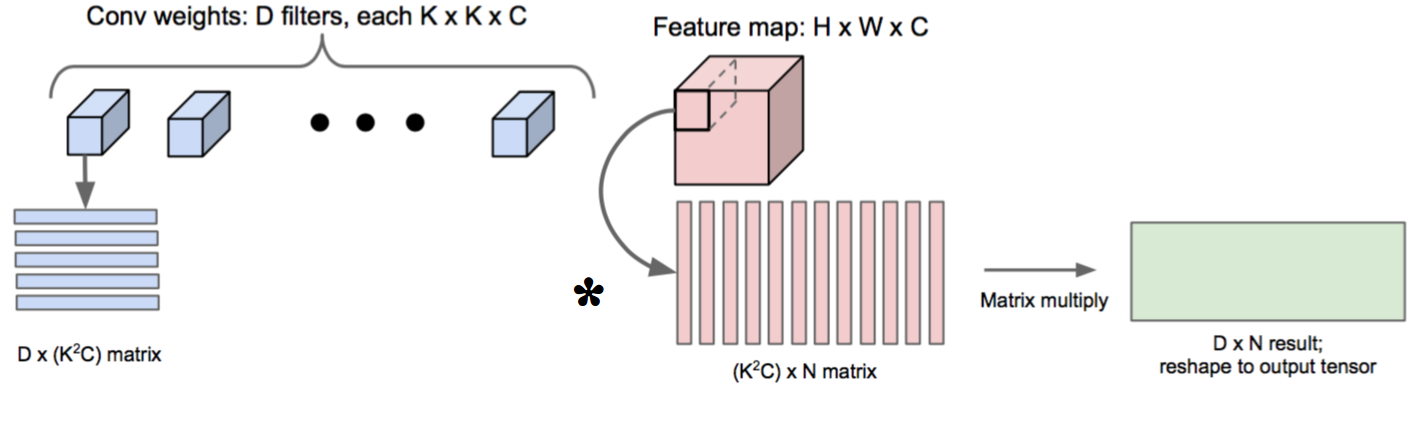
\includegraphics{Im2col.png}
\end{figure}

简而言之,im2col技术,每个窗口截取,将其展平,然后将它们堆叠为矩阵中的列。 再将内核展平
为行向量并在两者之间进行矩阵乘法,则在输出reshape后可以获得完全相同的结果。

Im2col 的简单伪代码表示如\ref{algo:im2col} 所示,

\begin{lstlisting}
\label{algo:im2col}
  def im2col(x, kernel_shape):
    # x is input activation
    rows = []

    # Assuming Padding = 0, stride = 1
    for row in range(x.shape[0] - 1):
        for col in range(x.shape[1] - 1):
            window = x[row: row + kernel_shape, col: col + kernel_shape]
            rows.append(window.flatten())
    return rows.transpose()
\end{lstlisting}

在im2col 方法中内存复制的复杂度为$O(MNC)$, 而卷积的复杂度为 $O(MNCk_1k_2)$,因此,在
大多情形下,内存复制所需要的时间开销同卷积本身相比仍然较低的,从而总体上im2col 可以实现
对于卷积操作的加速。另一方面,im2col 卷积的实现存在额外的$M\times N \times C$ 的内存
需求,这在移动端,嵌入式设备和其他资源严重受限的场景下往往是不太理想的。

\subsubsection{Memory Efficient Convolution}

MEC 方法\cite{Cho2017MECMC}作为对于im2col 的一种改进和扩展,旨在改善im2col 方法中对于内存的额外需求。
Im2col 实际是一种矩阵的降维手段(lowering scheme),将输入的3D 张量通过im2col可以转换
为 2D 矩阵并且可以直接使用BLAS 实现来完成矩阵乘法。Im2col 的方法变换之后的矩阵中存在着
相当多的数据冗余,这也表示这种方法可以通过去除这其中的数据冗余实现对于im2col 方法中过多
的memory overhead。Im2col 方法会将 $ W_i \times H_i \times C_i $ 的三维张量转换为 
$(H_f \times W_f \times C_i) \times (H_o \times W_o) $ 的二维矩阵,可见这一过程中,
额外需要的内存负担会随着问题规模存在平方级别的增长趋势。

同Im2col方法不同的是, im2col 方法中将输入的矩阵中的一个子块做降维,MEC 方法在实现的
过程中会一次将多列值降维,并且通过额外的矩阵乘法调用减少冗余的内存占用。

\begin{figure}
  \label{fig:mec}
  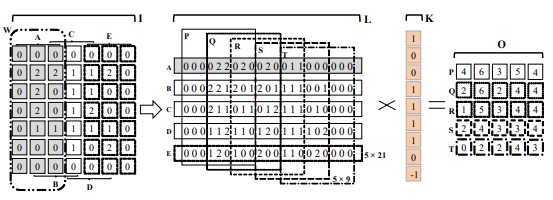
\includegraphics{mec.png}
\end{figure}

如图\ref{fig:mec} 中所示,对于一个 7x7 的输入,和3x3 的卷积核,这里需要实现降维的对象是
输入矩阵中的3列数据,记输入为 I,则这里需要将 $ I[0:7, 0:3] $ 这一区域中的数据平摊为一维,
即图中的第二步所示,依次按照滑窗实现输入的按照列的降维,在stride 为1 的情形下,这里在第二步
得到了降维后的 5 个一维向量,构成一个 5x 21的矩阵,而在实现矩阵乘法的过程中,则又需要
对于这个 5x21 的矩阵做划分为5x9 的子矩阵,在划分的过程中每向右移动三个单位(横向stride 乘
卷积核宽度)取一个子矩阵。每一个子矩阵和平摊(flatten)为一维向量的卷积核之间的乘积构成输出
的一行。 尽管这一过程中需要更多的矩阵乘法调用,但实际的乘法/加法操作则同im2col方法一致。
在计算复杂度上没有变化。

MEC 方法可以有效的减少im2col方法中在垂直方向上的数据冗余,在上图所示的计算过程中已经达到了
相对于im2col 方法54\% 的存储开销减少。这种方法甚至可以达到相对于im2col方法3.2 倍的存储资
源节省。

\subsection{快速卷积方法实现}

前面所提到的卷积算法,其优化的出发点都在于将卷积实现本身以高性能的角度解决问题(直接卷积方法),
或者说将卷积转换为研究相对充分的高性能计算问题(基于GEMM的方法),而对于卷积操作本身的复杂度
和运算量均没有实质性的降低。而卷积这一源自于信号处理的概念,则实际上在信号处理方法中已经有着
相当长远的研究,并且存在着很多可以实现卷积计算复杂性简化的方法,主要在于减少卷积实现中的乘法
操作。因此这一类方法被称为快速卷积方法。

\subsubsection{FFT 卷积}
对于信号处理中的场景而言,频域中的乘法对应于时域中的卷积。 使用DFT将输入信号转换到频域,再乘以滤波器的频率响应,然后使用Inverse DFT将输入信号转换回时域。
从傅立叶时代开始这种基本技术就广为人知。 但是,因为计算DFT所需的时间比直接计算卷积所需的时间长,所以使用傅里叶变换实现卷积的方法并没有受到足够的重视。
随着1965年快速傅立叶变换(FFT)的发展,这种情况发生了变化。 通过使用FFT算法计算DFT,与直接对时域信号进行卷积相比,通过频域进行卷积可以更快。而卷积的运算量
则获得了有效的缩减。一般而言,2维场景下,直接卷积的计算复杂度为 $O(n^4)$, 而FFT 卷积则可以将计算复杂度降低到 $O(n^2 \log_{2}n)$。而具体的在FFT 卷积
中的每一个步骤所需的计算复杂度同直接卷积方法的对比可以参考工作\cite{Mathieu2013FastTO}

基于FFT的卷积方法\cite{Zlateski2018FFTCA} \cite{Mathieu2013FastTO}可以表示为

\begin{align}
  f * g = F^{-1}(F(f)  \cdot F(g))
\end{align}
其中的$F$ 与 $F^{-1}$ 表示傅里叶变换和逆傅里叶变换,在离散场景下,$f$ 和 $g$ 需要具有相同数目的元素,这一点可以通过向两者中较短的那一方实现 zero padding实现。
DFT卷积的结果是一个循环卷积(circular convolution/ cyclic convolution),而从中获得有效的卷积结果仍然需要从循环卷积的结果中抽取其中的最后 $|f| - |g| + 1 $
个元素。

在FFT 卷积方法中,卷积的输入和权重在经过离散傅里叶变换之后被变换为复数表示,而此后则需要执行二者之间的复数矩阵乘法。而在这一过程中,又具有着以下两种
特性能够进一步降低乘法操作的数目。

\begin{itemize}
  \item 实数值傅里叶变换的 Hermitian 对称性;
  \item 快速复数乘法计算;
\end{itemize}

实数域中的信号的 FFT 变换是具有 Hermitian 对称性(Hermitian symmetry)的, 即实数矩阵在傅里叶变换之后的矩阵同其共轭转置矩阵(conjugate transpose)是相等的,
这使得在 FFT 卷积方法中的矩阵乘法部分的实际有效乘法量可以进一步减半。一个尺寸为 $m x m$ 的实数值矩阵的离散傅里叶变换由于 Hermitian 对称性可以用 $ m x (floor(\frac{1}{2} + 1)) $ 
个复数来表示。同时又由于 $ U^H V^H = ( UV )^H $,矩阵乘法结果中的一半元素的值(上/下三角)可以通过取已计算值的共轭获得。

\paragraph{复数乘法计算}
复数计算在信号处理中有着广泛的应用,然而不幸的是,很多现代硬件在底层的指令上则缺少直接计算复数计算的支持,这使得复数计算的实现不得不面临着额外的挑战和付出。
而针对于ARM平台,尽管在ARMv8.2指令集(ISA) 之后添加了 FCADD (Floating-point Complex Add), FCMLA (Floating-point Complex Multiply Accumulate) 操作,
然而实现这一指令集的芯片微架构(microarchitecture)并不占据主流,主要集中在高端智能收集芯片上,比如苹果应用于iPhone X上的A11芯片及其之后的应用于iPhone XS系列的
A12芯片以及iPhone 11 的 A13芯片,在很多的嵌入式设备场景下的low profile的计算资源场景下,指令级别的复数操作支持仍然是缺失的。

一般的复数乘法中,一对复数相乘需要四次复数乘法,即

\begin{align}
\label{eq:complex_mul}
  (u_r + i u_i) (v_r + i v_i) = u_r v_r - u_i v_i + i ( u_i v_r + u_r v_i )
\end{align}

而对于\ref{eq:complex_mul} 稍加变换既可以得到复数乘法的快速算法,该方法只需要三个实数乘法。

\begin{align}
\label{eq:complex_mul_fast}
  (u_r + i u_i) (v_r + i v_i) &= [ u_r v_r - u_i v_i, i(u_r v_i + u_i v_r)]
                               &= [ u_a - u_c,i( u_a + u_b) ]
\end{align}

where 
\begin{align}
u_a = v_r ( u_r + u_i )
u_b = u_r ( v_i - v_r )
u_c = u_i ( v_r + v_i )
\end{align}

这一方法,通过使用更多的加法实现在复数乘法计算过中乘法的减少 。

\paragraph{快速复数乘法在傅里叶卷积中的应用}

在执行图像块的变换后,产生一个复数张量 $U = U_r + i U_i$ ,可以计算实值张量 $U_r + U_i$ 并将其与Ur和Ui一起存储。 类似地, 卷积核权重在离散傅里叶变换之后得到一个
复数张量 $V = V_r + i V_i $, 张量 $V_i - V_r$ 和 $V_r + V_i$ 可以在内核变换期间计算, 并与 $V_r$ 一起存储(不必存储$V_i$ )。这里每个变换前的实数域的输入
对应于变换后的三个实数值,而不是直观理解上的每个变换后的值对应两个用来表示复数实部和虚部的两个实数。 然后,可以用三个独立的实值张量的元素间乘积替换复数张量的
元素间乘积. 而由此计算得到的三个 实数张量则可以在计算逆变换的过程中被隐式的转换为单个实数张量。总体来讲,快速复数乘法的实现,可以使得原本的复数域中的一个矩阵间
乘法转换为3个实数域中的矩阵乘法, 同直接计算复数乘法相比,可以将乘法的操作数减少 25\%.

FFT 卷积在执行计算的过程中需要将权重填充到和输入同等大小,这回导致额外并且不必要的内存负担,特别是在
卷积核本身毕竟小的状态下。信号处理中对于这一问题也有着比较成熟的解决方案,即 overlap add 和 overlap save
方法。切换到深度学习的场景下,可以实现对于输入的图像的切分,在每个小块上执行FFT 卷积,再将得到的结果
通过类似overlap add / overlap save的方法拼凑为整个图像输入的结果。 但是,这样的方法还需要将内核权重
填充到合适的大小(通常为2的幂)以达到最优性能。 即使将内核权重填充到架构寄存器大小的较小倍数(例如8或16)
,也会导致内存需求增加7到28倍。 此外可以通过动态执行FFT, 将FFT作为卷积层计算的一部分来最小化这种额外填充
卷积核权重并将其转换到频域的overhead。 但是,这会产生大量的性能开销,使得资源受限的嵌入式设备雪上加霜。


\subsubsection{Winograd 卷积}

Winograd minimal filtering算法是在信号处理中常用的一类快速算法,并且在信号处理领域已经有了相当时间的应用和研究。而
\cite{Lavin2015FastAF} 则将这一方法引入卷积网络的计算中。下面将从卷积网络计算的角度,考虑这一算法在
卷积计算中的具体应用场景,简要解释介绍Winograd 算法对于卷积计算过程的优化。

从1D 的卷积过程来考虑,对于卷积核大小为3 的情形,对于连续两次的卷积过程,如图\ref{fig:conv_slide}
所示,输出 $r_0$ 由输入$k_0, k_1, k_2$ 同卷积核参数做元素间乘法相加得到,同样的,输出中的 $r_1$ 
则由输入$k_1, k_2, k_3$ 计算得出,这一过程中输出两个值需要有4个输入,将这一过程用矩阵乘法来做表示

\begin{figure}
\label{fig:conv_slide}
  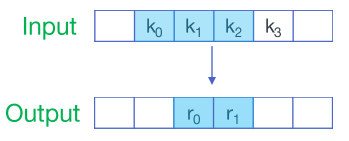
\includegraphics{conv_sliding.png}
\end{figure}


\begin{align}
  \begin{pmatrix}
    k_0 & k_1 & k_2 \\
    k_1 & k_2 & k_3 
  \end{pmatrix}
  \begin{pmatrix}
    w_0\\
    w_1\\
    w_2
  \end{pmatrix}
  =
  \begin{pmatrix}
    r_0 \\
    r_1
  \end{pmatrix}
\end{align}

直接做矩阵乘法,这一过程需要 6 次乘法和 4次加法:

\begin{align}
  r_0 = k_0 w_0 + k_1 w_1 + k_2 w_2 \\
  r_1 = k_1 w_0 + k_2 w_1 + k_3 w_2 
\end{align}

而如果对上述的乘法计算过程做如下的变换:

\begin{align}
\label{eq:winograd_mul}
  \begin{pmatrix}
    k_0 & k_1 & k_2 \\
    k_1 & k_2 & k_3 
  \end{pmatrix}
  \begin{pmatrix}
    w_0\\
    w_1\\
    w_2
  \end{pmatrix}
  =
  \begin{pmatrix}
    m_0 + m_1 + m_2 \\
    m_1 - m_2 - m_3
  \end{pmatrix}
\end{align}

其中,

\begin{align}
  m_0 = (k_0 - k_2) w_0
  m_1 = (k_1 + k_2) \frac{w_0 + w_1 + w_2}{2}
  m_0 = (k_0 - k_2) w_0
  m_2 = (k_2 - k_1) \frac{w_0 - w_1 + w_2}{2}
\end{align}

由于在卷积的过程中,卷积核权重的值都是确定的,所以其中 $m_1, m_2$中同 $w$ 相关
的这一部分均可以在计算矩阵乘法(卷积操作)之前预先计算。从而这一过程可以将
乘法的数目减少到4次,而上述的这一过程即为 $F(2, 3)$ 卷积在1D 场景下的实现,
而二维的场景,只需要将1D 的场景做进一步的嵌入即可实现。

具体而言,对于如图所示的 $F(2x2, 3x3)$ 的场景
\begin{figure}
\label{fig:conv2x2_3x3}
  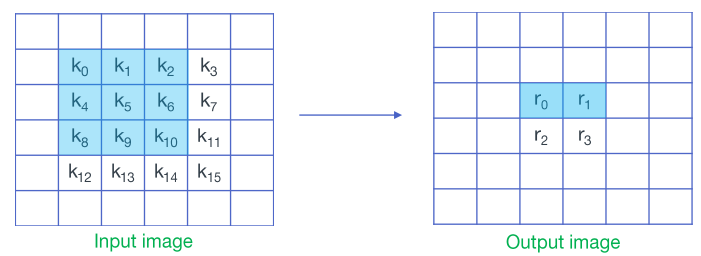
\includegraphics{conv2x2_3x3.png}
\end{figure}

用矩阵乘法的形式表示这一卷积过程

\[
\label{eq:f2x3}
  \begin{pmatrix}
    k_0 & k_1 & k_2 & k_3 & k_4 & k_5 & k_6 & k_7 & k_8 & k_9 & k_10 \\
    k_1 & k_2 & k_3 & k_4 & k_5 & k_6 & k_7 & k_8 & k_9 & k_10 & k_11 \\
    k_4 & k_5 & k_6 & k_7 & k_8 & k_9 & k_10 & k_11  & k_12 & k_13 & k_14 \\
    k_5 & k_6 & k_7 & k_8 & k_9 & k_10 & k_11 & k_12 & k_13 & k_14 & k_15
  \end{pmatrix}
  \begin{pmatrix}
    w_0 \\
    w_1 \\
    w_2 \\
    w_3 \\
    w_4 \\
    w_5 \\
    w_6 \\
    w_7 \\
    w_8
  \end{pmatrix}
  = 
  \begin{pmatrix}
    r_0 \\
    r_1 \\
    r_2 \\
    r_3
  \end{pmatrix}
\]

类比于 1D 场景下的处理方法,这里可以得到相似的处理形式,不同点在于,1D 场景下简化
的乘法\ref{eq:winograd_mul}中表示的值均为Scalar,而2D场景下对应的值为一个子矩阵,
可见在2D 场景下,乘法操作的数目可以由直接矩阵乘法计算的36次,减少到16次,从而以
乘法计算的复杂度来考虑,可以达到 2.25 倍的复杂度降低。

\section{神经网络量化研究}

减小计算资源的需求并提高功耗利用是在边缘设备上实现智能应用的一大挑战。量化方法
便是解决这一挑战的一条可行的途径。量化过程做一个简单的比喻,可以理解为是图片的
编码,现实世界中的图像视觉信号是连续的模拟信号,量化过程便是使用有限的编码位数,
用离散的整数值逼近重建实际的连续值。

在机器学习应用中,神经网络由激活节点,节点之间的连接以及与每个连接关联的权重参数组成。
这些权重参数和激活节点计算可以量化。在硬件上运行神经网络往往存在着数百万的乘法
和加法运算。 具有量化参数的低位数学运算与对神经网络的中间计算进行量化相结合,
可带来较大的计算增益和更高的性能。

\subsection{网络模型量化方法}
量化网络模型在很多应用场景下的存在精度下降的问题,为实现在嵌入式场景,移动场景等
边缘设备的高效模型部署和智能应用处理,近些年也有很多研究着力于实现使用低位数的模型
(low-bit model)低精度的数据表示(low-precision representation)在对应的机器学习
任务上获得较高的精度指标。 相当多的工作在着力实现量化对整个网络准确性的影响最小。
量化背后的核心思想是神经网络对噪声的弹性或者说容忍性。 尤其是深度神经网络,
经过训练可以识别 关键模式并忽略噪声。 不逊于全精度(full precision)网络的准确度
加上显着减少的内存占用, 功耗和计算速度的提高,使量化成为将神经网络部署到嵌入式
硬件的有效方法。

而在网络训练结束之后单独对于网络权重做量化(post-training quantization)处理,这一网络量化处理最为直观和朴素的
方法对于较大的网络模型一般实现的实际精度效果仍然是可接受的,而对于参数比较小的
模型,这种方法则会造成相当的精度损失。参数较大的模型具有更丰富的表达能力,同时
抗噪性也更强,而小模型本身的模型表达能力便受到容量的限制,参数量化过程则会对模型
的表现能力造成巨大的波动。网络模型中参数的分布可能会存在比较极端的情形,这可能
存在于同一个卷积操作的不同输出channel 中,也可能存在于网络中不同的层次中。
这使得我们在实现有限位数的量化的过程中,权重差距比较小的部分会存在较大的量化
误差。另外一方面,这种直接的量化策略下,离群点对于整体量化的效果会存在比较明显的影响。

工作\cite{Jacob2017QuantizationAT}中在模型的训练部分,提出了可以在模型训练的
过程中模拟量化效果,从而填补模型训练和模型量化之间所存在的gap。这一文中描述了
目前通用的执行网络中端到端整数计算的策略,并且提出在网络的训练过程中可以在计算
节点间插入 Fake Quantization 操作,使得网络在前向推理的过程中,效果上执行的是
端到端的整数计算过程,而网络本身的权重参数仍然为浮点数,从而网络反向梯度更新仍然
可以像普通的训练过程一样执行。

\cite{Louizos2019RelaxedQF} 为了训练可以有效离散化而又不损失性能的网络,引入了
可微分的量化过程。通过将权重上的连续分布和网络的激活转换为量化网格上的分类分布,
可以实现可区分性。随后将它们放宽(relaxed)为连续值替代,从而可以进行基于梯度的
有效优化。

\subsection{模型量化计算实现支持}

诸如 TensorRT,TensorFlow,PyTorch,MxNet等框架均在不同程度上具有了处理量化
网络模型的能力。一些模型的计算过程中会包含量化和反量化操作,即量化计算的过程
并不是端到端的,即网络中某个操作(通常是如全连接或者卷积这种计算密集型操作)
的输入仍然是32位浮点数,在执行该操作之前,可以通过量化操作将对应的输入转换为
8位整数表示执行计算,最后再将计算的结果反量化回32位浮点表示,这种量化计算方法
在多个连续的网络计算操作的进行过程中,可以通过去除计算流程(computation flow)
中的冗余的量化/反量化操作达到将浮点运算转换为定点计算(即整数型计算),从而使得
输入的32位浮点表示的特征在经过一次变换之后,通过多个支持整数计算的操作,最终
在输出前再反量化为浮点表示。而这一流程的优势也仅仅存在于,计算流程中的每一步
都需要支持整数型计算,否则将会引入额外的量化/反量化过程,使得计算整体的效率
得不偿失。

这些深度学习网络框架对于机器学习从业者而言,很多都只是定义了计算的接口,而真正
的计算则是由支持PyTorch, TensorFlow 等框架的底层的kernel library来实现的,
这些计算库才是真正执行深度模型计算的work horse。而计算库的实现也是同执行运算
的硬件平台密切相关的。就CPU上的量化计算而言,在Intel x86芯片架构的桌面和服务器端,
Intel MKL(Math Kernel Library) 提供了各种针对硬件高度优化的数学计算支持,同时
也包括整数型的矩阵乘法和卷积实现
而且同时针对于近些年来普遍应用于深度学习视觉任务中的小尺度卷积而言,在Intel
硬件平台则由LIBXSMM\cite{Heinecke2016LIBXSMMAS} 实现针对性的计算优化。顾名思义,
这里的XSMM 即指在x86 平台的小尺度矩阵乘法计算(Small Matrix Multiplication)而在
LIBXSMM 的小尺度卷积实现中,则是对比于FFT方法转换到频域做计算的方法,在小尺度
的情形下直接卷积操作在针对性优化下可以有更为高效的表现,因此这里的卷积算法采用了
直接卷积计算。同时LIBXSMM 支持 十六位整数和8位整数的计算。

而Facebook 则专门针对于深度网络的量化计算推出QNNPACK,实现在ARM 移动平台和
x86 桌面端的量化网络计算需求,而其中的卷积计算方法则是采用了 Indirect Convolution
\cite{Dukhan2019TheIC}(一种im2col 方法的变种,从计算实现角度改善memory overhead)。
另外,在服务器端的CPU 低精度模型推理优化计算。FBGEMM 的实现中采用了和QNNPACK中
类似的im2col 改进策略。GEMM 方法实现的卷积很大程度上依赖于高性能计算研究中对于
矩阵乘法的优化,然而HPC 毕竟同深度学习模型推理之间是存在着不匹配的. 很多HPC 库
并不提供针对于量化场景的相关计算,HPC 针对的场景往往时大规模的矩阵计算,甚至是
规模大到需要在分布式集群执行的计算,而没有针对于深度学习中的很多矩阵的计算,特别是
近些年来的小尺度的矩阵的计算做优化,因而不能充分利用到深度网络权重矩阵的特性。

% \section{ARM 架构上的神经网络计算}

% !TeX root = ../main.tex

\chapter{图表公式例子}
\label{cha:chapter02}

\section{整数快速卷积实现}

Winograd 卷积的一般过程包括输入变换(input transform),权重变换(weight transform),矩阵乘法(GEMM)以及输出变换(output transform)。
其中权重的变换只用操作一次,便可以在不同的输入复用。一般考虑到运行时效率,权重变换可以在卷积操作实际执行前操作,从而Winograd 卷积的实际执行过程可以概况为
以下步骤:
\begin{enumerate}
  \item 将输入的图像块转换到 Winograd 域
  \item 执行在 Winograd 域中执行变换后的输入和权重的矩阵乘法
  \item 将矩阵乘法的结果转换回空间域
\end{enumerate}

若使用F(m, r)有m个输出的r-tap FIR滤波器,F(m, r) 接收的输入的大小为 ( m + r - 1), 则 Winograd 卷积算法可以表示为

\begin{align}\label{eq:winograd1d}
  Y = A^T [(Gg) \circ (B^Td)]
\end{align}

在式 \ref{eq:winograd1d} 中,$\circ$ 表示 Hadamard Product.

Winograd 卷积算法中的矩阵乘法量同输入的尺寸一致,即 $F(m, r)$ 的Winograd 卷积,其中需要执行 m + r -1 个乘法。而更高维度的Winograd 算法 $F(mxn, rxs)$,则可以通过
在对应的 维度嵌套一维的卷积算法\ref{eq:winograd1d} $F(m, r)$ 和 $F(n, s)$ 实现。特别是对于卷积网络中,最为广泛使用的方形滤波器,即卷积核的宽高相等,$F(m x m, r x r)$
表示卷积核尺寸为 $r x r$,对应的输出尺寸为 $ m x m$, 二维的 Winograd 算法可以表示为 :

\begin{align}
\label{eq:winograd2d}
  Y = A^T [(GgG^T) \circ (B^TdB)] A
\end{align}

而与之对应的直接卷积方法中对应的矩阵乘法则为 $m^2r^2$ (输出为$m^2$个,每个输出对应着$r^2$个输入,每个输入都要同filter中的对应值做一次乘法),而这里二维场景的
Winograd卷积实现,其中的乘法操作的规模为 $( m + r - 1)^2$。而在卷积算法的实现中,矩阵乘法(GEMM)无疑是最为占据主导的操作,自然也是效率优化的瓶颈。于是,以乘法的
规模作为复杂度的度量,Winograd 卷积相对于直接卷积方法,实现的复杂度简化为

\begin{align}
  \label{eq:winograd_reduction}
  \frac{m^2r^2}{(m+r-1)^2}
\end{align}

因此,对于较为常用的两类Winograd 卷积实现 F(2, 3), F(4, 3),即卷积核大小均为3,输出的尺寸分别为2和4的卷积,理论上分别可以达到2.25 和 4倍的加速。而在实际的实现中,
还需要考虑到对于输入和输出的变换所带来的额外开销,在卷积的规模,特别是矩阵乘法的规模没有达到一定的限度时,Winograd卷积方法不一定能够实现理论的加速值。
尽管使用更大尺度(输出的尺度和卷积尺度)的Winograd 卷积可以实现更大程度的复杂度简化,但同时也受限于变换过程的数值稳定性,更大尺度的 Winograd 卷积一般也
意味着不准确,可能会存在精度的损失。

另外,关于Winograd 卷积中使用的变换矩阵 $G$, $B^T$, $A^T$ 的具体表示的推导可以通过Cook Toom 算法来实现。具体过程可以概述为,使用拉格朗日插值多项式,将相当于卷积
的多项式乘法,转换为多项式在固定数目的插值点处取值的逐元素乘法。 Cook-Toom算法的缺点是,随着变换大小的增加,变换很快变得不稳定。 但是,它们非常适合卷积神经网络中使用的3x3小卷积。

Winograd快速卷积算法的更一般形式是使用中国剩余定理。 Cook Toom 算法只是其中之一。而这一过程的具体不在本文的范畴,有兴趣的可以参考 Fast Algorithm for Convolutional 
Neural Networks 中的补充材料(https://github.com/andravin/wincnn/blob/master/2464-supp.pdf)。


快速卷积算法相对于直接卷积和基于GEMM的卷积(比如im2col,im2row等)的实现的主要一大优化目标在于减小运算中乘法的规模,尽管快速卷积方法往往为实现减少乘法的次数而不惜引入
一些额外的加法操作以及对于输入的变换,但在运算中乘法操作达到一定的规模后,乘法数目减少所带来的计算收益是可以超过这些额外的开销的。值得注意的是,快速卷积方法中为减少乘法
操作而不惜引入加法的这一优化手段,并不是因为加法操作会比乘法操作快,这个概念具体到现代的硬件设备上的乘法和加法实现实际上往往是站不住脚的,而实际上在现代硬件设备中
乘法和加法操作往往是可以聚合(fused)在一起的,也就是乘累加(multiply & acculate)操作。从而即使额外引入加法,在仔细设计算法执行后,在具体的硬件实现中,也不会带来
额外的计算开销。

而另外一方面,作为另外一种更为常用的快速卷积方法实现,快速傅里叶变换(FFT)方法在整体的形式上同Winograd 方法\ref{eq:winograd1d}类似,
其中的变换过程则会对应为FFT和inverse 类似,其中的变换过程则会对应为FFT和inverse
 FFT,即变换矩阵$G$ 和 $B^T$表示FFT,而$A^T$ 则表示inverse FFT。同时,式\ref{eq:winograd1d} 中的也将对应的修改为复数乘法,同实数乘法不同的是,直接的复数乘法需要
 4 次实数乘法来实现。然而,卷积网络中的输入往往都是实数,而实数的傅里叶变换存在Hermitian对称性,从而可以将矩阵复数乘法的复杂度减半,只需计算矩阵中的一半的值,另外一半
 只需要取对应的已计算值的共轭复数即可。但即便如此,FFT卷积实现中仍然需要达到 64x64 的输入尺度才能在乘法规模的优化程度上达到和 Winograd 卷积 F(4, 3) 在输入为6x6 时的
 同等水准,使用FFT实现卷积操作的加速需要相比于Winograd卷积更大的内存需求,

 下面对于卷积实现中的一些符号做如下约定。卷积操作作用于输入特征的局部,并且局部特征的卷积结果输出也仅由这一局部的输入所决定。对于输入局部(input tile)尺寸位 $m x m $,
 卷积核(kernel)尺寸为 $k x k$ ,输出块(output tile)特征大小为 $ r x r $ 的卷积操作,可以记为 $ F(r\times r, k\times k, m\times m) $ .

 \subsection{数据排布}

 卷积网络中常用的数据排布方式(data layout)存在 Channel First 即 NCHW 和 Channel Last 即 NHWC 。而对应的在数据加载的过程中,由于在ARMv8-A 架构下,存在 32 个128位
 SIMD 寄存器,因此每个寄存器可以用来存储 4 个32位整数(int32)或者 16 个8位整数(uint8)或者 8个16位整数(int16)。以32位整数举例,在NCHW 数据排布下,在完成128位的
 数据加载后,一个SIMD 寄存器可以用来储存矩阵中一行的四个值,而在NHWC 数据排布下,同样的单个SIMD寄存器可以用来加载矩阵中位于同一个位置的连续四个通道(channel )的值。
 而在Winograd 快速卷积的实现中,NHWC 的数据表示是具备着实现灵活性上的相当的优势的,特别是在量化计算的场景下,定点(fixed point)表示的数据在计算过程中会频繁涉及数据
 位长(data width)或者说数据精度(precision)的变换,NHWC的表示可以灵活的实现并行算法。同时在考虑不同规模的算法下,NHWC的data layout 也可以实现寄存器的高效利用。
 下面在具体的Winograd 卷积的实现中会做对比和具体的说明。

\section{F(2x2, 3x3, 4x4) 的卷积实现}

\subsection{Winograd变换及逆变换}

Winograd 卷积输入变换最为常用的特征方程是

\begin{align}
  X^T x X = 
  \begin{pmatrix}
    1 & 0 & -1 & 0 \\
    0 & 1 & 1 & 0 \\
    0 & -1 & 1 & 0 \\
    0 & 1 & 0 & -1 \\
  \end{pmatrix}
  x
  \begin{pmatrix}
    1 & 0 & 0 & 0 \\
    0 & 1 & -1 & 1 \\
    -1 & 1 & 1 & 0 \\
    0 & 1 & 0 & -1 \\
  \end{pmatrix}
\end{align}

在这里输入变换的输入特征x 无论是 NHWC 表示还是 NCHW表示,抛开Channel 维度而言,矩阵在平面表示上都是row major 的,即同一行中的元素位于矩阵表示中的更内层。而矩阵x
左乘一个矩阵可以表示为 x 中的行元素的线性组合(这一点会在矩阵乘法一节详细展开说明)。上述矩阵的变换过程可以分为两步:

\begin{itemize}
\item 第一步计算 $X^T x $。这里可以借助矩阵 $X^T$ 的简单形式和矩阵左乘的特性快速实现。
\item 第二部计算 $X^T x X = (X^T(X^T x)^T)$,可见这一计算过程只需将第一步的计算结果转置,再重复第一步的计算过程,最终再将结果转置。
\end{itemize}

在这里简单讨论以下NHWC 表示和NCHW 表示在这里对于这一计算过程的影响。首先使用 NCHW 表示,则一个SIMD 寄存器中将包含处于矩阵中同一行的元素,在实现输入特征同
变换矩阵的乘法中将深度依赖矩阵左乘时,其中行的线性组合性质。同时由于这种数据表示,上述算法中的转置操作也不可避免,而转置操作在硬件实现上则是代价相对较高的一种
操作;更重要的一点是,在量化计算中,NCHW 的表示会为算法设计带来更多的困难,比如这里的输入变换中,如果输入的数据类型是 32 位整数(int32),则在ARMv8-A 中的
SIMD 计算中,可以用 4 个 128位的寄存器来存储一个 4x4 矩阵的值,计算过程和上述的数学表示相差无几。而如果输入的特征是 8 位整数(uint8),则上面的算法就需要重新
设计,或者说,NCHW的数据表示下,不得不针对每种类型的数据重新设计算法。最后,如果考虑到后续的计算,NCHW 表示的计算结果中位于同一寄存器中的值必须分散(scatter)
到不同的位置来实现矩阵乘法,而在NHWC 的布局下,每个寄存器都是同一位置不同channel 的值,对于输入变换过程,可以使用  16个 SIMD 寄存器来表示算法中的 4x4 矩阵,
这一表示允许更加灵活的使用SIMD实现对不同channel 的数据的同步计算,而不必针对于输入数据的位长而重新设计算法,数据位长或者精度只会改变SIMD 计算中可以同时操作
的channel数目,数据位长越低,则能同步处理更多channel的数据,同一个128位的寄存器,可以同时处理4个32位的整数或者8个16位的整数。 

此外,NCHW的data layout 的影响还会受限于变换算法过程中的矩阵大小,$F(3, 2)$ 的情形下矩阵是 4x4 的,而在 $F(3, 4)$ 的场景下,输出的矩阵则是 6x6 的。  如果
使用 NCHW 的表示,这样将会使得寄存器中存储一个6x6 的矩阵变得十分棘手。在32位整数的情形下,需要一个半寄存器来表示6x6矩阵中的一行,这样便只能在算法的过度设计
和寄存器的浪费中二选一了。

在量化计算的场景下,这里输入的特征为被量化后的8位无符号整数,执行16次数据加载之后可以获得 4x4 的输入矩阵,ARMv8-A NEON指令中支持一次加载一个64位寄存器
或者一个128位寄存器,实现中采取一次加载8个8位无符号整数(一个64位寄存器),即这里实际加载到的输入是4x4x8 的。同时在这里考虑到定点计算过程中的溢出的影响
需要将8位整数转换为16位整数,而转换为16位整数之后,同一位置的多个channel的数据刚好占满一个128位的寄存器。最终变换输出的结果也是由16位带符号整数表示。

而对于权重变换而言,在通用的Winograd 卷积变换中,同上述输入变换所对应的权重变换矩阵G 为 
\being{align}
G = 
\begin{pmatrix}
  1 & 0 \\
  \frac{1}{2} & \frac{1}{2} \\
  \frac{1}{2} & -\frac{1}{2} \\
  0 & 1
\end{pmatrix}
\end{align}

为实现这一计算过程的整数化,只需要对这一矩阵扩大两倍即可,即用于整数计算的权重变换矩阵为

\begin{align}
  \begin{pmatrix}
    2 & 0\\
    1 & 1\\
    1 & -1\\
    0 & 2
  \end{pmatrix}
\end{align}

同时,对应的,由于在权重变换的过程中$G $和$G^T $ 均乘2,所以在最终的输出变换过程中需要对输出值除4。

输出变换矩阵$A^T$ 则仍然使用
\begin{align}
  A^T = 
  \begin{pmatrix}
    1 & 1 & 1 & 0 \\
    0 & 1 & -1 & -1
  \end{pmatrix}
\end{align}

\subsection{矩阵乘法实现}

在输入和权重均经过Winograd 变换之后,变换后的矩阵会执行元素间的乘法,然后将对应位置的乘积结果累加(element-wise addition of Hadamard products)。
表示输出通道为m,输入通道为c的权重值可以在c通道中的所有输入区域被复用,
而 c 通道中位置为 $(i, j)$ 的输入则在所有的$(i,j )$位置输出的区域被复用。 这一观察表明,实际上这一操作本身可以转化为研究较为充分的通用矩阵乘法(GEMM)。
对于输入的channel数为 C,输出的channel数为M,且具有R 个分块的卷积, 在 $F(2, 3)$ 的Winograd 卷积中输入的元素为16个,那么对应的需要执行16 次 $[RxC]x[CxM] $
的矩阵乘法。


\subsubsection{矩阵在内存中的灵活表示}
矩阵在存储空间中是以一整块连续的存储块空间所表示的。在矩阵的存储(storage)中有两个同内存(memory)相关的的关键问题:维度(dimension)和跨度(stride)。

跨度是指在遍历矩阵的过程中,在通过不同维度的过程中需要跨过的字节(bytes)数。跨度的存在可以使得很多矩阵的处理变得更加快速有效,同时,对于跨度的理解也有助于
更加容易的理解矩阵操作的实现。矩阵存储在被成为data buffer 的连续(contiguous)的同质(homogeneous)内存块( block of memory)中。Strides 可以作为一个
矩阵的meta data(元数据)实现多维矩阵之中的不同维度的index(索引)与它在连续memory block中的位置的映射(mapping)。简而言之,strides表示对于每个维度
的连续元素之间的字节间距(byte-separation)。同时矩阵存储空间的同质性也保证了矩阵在存储空间中的连续元素间的单位距离的一致性,比如对于int32类型的矩阵,
这里计量矩阵元素的单位距离就是 4个bytes,每两个矩阵元素在存储中的距离为4。于是对于多维矩阵而言,比如对于int类型的二维矩阵 $A$,$A$ 在矩阵表示的最内侧
的元素在memory中连续存储 ,即二维矩阵中的column(列)元素在实际的存储中相邻,在二维场景下可以成为 row-major。从$A[0, 0]$所表示的元素
移动到$A[0,1]$所表示的元素,即在同一行(第0行)中的元素间,从第0列移动到第1列,这里需要在data buffer中移动4个byte,也就是在列所对应的维度上的一个stride。
然而,如果从$A[0,0]$ 所表示的元素的位置移动到 $A[1, 0]$, 即在同一列(第0列),移动到下一行(从第0行移动到第1行)所在元素的位置,直观而言,需要先遍历
这一行中剩余的元素,才能够到达下一行,然后再下一行中遍历元素到达目标元素,比如矩阵$A$是一个$3x3$大小的矩阵,那么从 $A[0,0]$ 到$A[0,1]$ 需要遍历
$3x4$ 个bytes。也就是说矩阵$A$在行的维度上相邻元素间的间距(row stride)是 12个 bytes。Stride 的存在可以使得矩阵的处理变得更加灵活,也使得很多矩阵操作轻量化,矩阵的转置
以及reshape等操作可以不用实际操作矩阵,而仅仅是改变矩阵各个dimension 所对应的stride这一meta data,比如矩阵的转置实际上可以只是交换对应的stride并且
改变矩阵的shape信息。比如,对于前面例子中的3x3矩阵$A$,假如这里使用$(12, 4)$表示矩阵 $A$在第0维度(row)的stride为 12 个bytes,而在第1维度(column)
的stride为 4个bytes。它的转置$A^T$并不需要对于$A$所对应的内存块中的元素做实际的重新排布 (reorder),而只需要将 $A$原本所对应的stride信息修改为
$(4, 12)$ 即可。同样的,在考虑到矩阵的stride这一元信息(meta info)的场景下,对于举证的处理也不能直观的认为矩阵的最内层(innermost)元素之间的距离
一定是单位该元素数据类型的尺度。而是在沿着矩阵的某个维度实现遍历处理的过程中,这一维度上对应元素间的距离一定是这一维度队对应的stride。

除其他外,基于原有的矩阵的创建一个新的矩阵对象的操作也可以因此而轻量化。创建一个新的数组元数据,该元数据使用相同的data
buffer 来创建该数据缓冲区的新视图,该视图对缓冲区的解释(interpolation)不同(例如,形状,偏移量,字节顺序, 大步等),但共享相同的数据字节。 例如slice 操作,
只需要创建一个新的矩阵元数据信息,对应的更改其起始位置的offset和各个维度的stride,而不需要从memory中拷贝data buffer中的相关数据元素。

\subsubsection{ARMv8-A 架构硬件特征}

ARMv8 指令集架构的设计中包含 32个64位 (doubleword)NEON 寄存器,或者称为 D 寄存器,同时,这32个 D 寄存器也可以视为 16 个 128位(quadword)寄存器,
称为 Q 寄存器。

NEON 作为一个SIMD 并行计算的协处理单元,具有以下流水线执行特征
\begin{itemize}
\item NEON指令运行在其独立的10-stage 的流水线中
\item ARM 在每个执行周期(cycle)可以调度(dispatch)两个NEON 指令
\item 可以容纳16条指令的指令队列(16-entry instruction queue)可以用于在指令实际进入pipeline之前作为缓冲
\item 可以容纳12条数据记录的队列用于存储ARM 寄存器的值,在ARM调度指令之后保存当时ARM 寄存器的值
\end{itemize}

由于以上的特征,在实现ARMv8 指令集的大多架构下,由ARM到NEON(由CPU 处理器到 SIMD 协处理器)的数据传输是相对高效迅速的,而由NEON到ARM 的数据传输则相对
有较高的延时(latency);
同时在ARM 处理器一方不会因为 NEON 协处理器的执行而停滞,除非NEON 协处理器的队列已满。ARM 处理器可以向 NEON 协处理器调度分布一系列的指令后继续处理器
本身的任务,直到NEON 指令的结果返回;
另外,NEON 指令的实际执行同在编写代码中直观观察到的执行并不是一致的,由于队列的存在,NEON 指令的实际执行是有所延后的。这就导致,如果由程序修改了另外一个
程序所需要的缓存行(cache line),会导致ARM 处理器侧的停滞,直到NEON的执行同步。

\subsubsection{硬件相关的矩阵乘法性能优化}
矩阵操作通常是最难实现的,部分原因是潜在解决方案的空间非常之大。 

一个简单的程序,它实际的执行性能起始同硬件架构的环境有着复杂的联系。硬件环境或者程序之中细微的改变可能会对代码的执行效率带来极大的改变。嵌入式场景和
科学计算特别是机器学习领域相关的计算都是需要特别关注代码的执行效率的,因此,必须针对性的对于硬件架构编写高效的程序。尽管实际的硬件环境是及其复杂的,
但在设计硬件相关的高效计算中,仍然存在着相对通用的模型和指导方针。比如提高缓存性能的一大方法,blocking 技术。

定义两个矩阵 $A$, $B$, 对应的尺度分别位 $m x k$, $k x n$, 记为 $A(m, k) $ 和 $ B(k, n) $, 则两者的矩阵乘积可以表示为

\begin{align}
  C(m, n) = A(m, k) x B(k, n)
\end{align}

直观而言,矩阵乘法可以视作是矩阵A 中的行同矩阵 B 中的对应的列的点积的集合,是对应矩阵元素的乘积的和(sum of element-wise multiplication)。简单的伪码
实现如下:

\begin{listing}
\label{code:matmul_naive}
  for (int i = 0; i < m; i++) {
    for (int j = 0; j < n; j++) {
      for (int p = 0; p < k; p++) {
        C(i, j) += A(i, p) * B(p, j);
      }
    }
  }
\end{listing}

对这一简单直接的矩阵乘法的实现的可视化可如下图所示

\begin{figure}
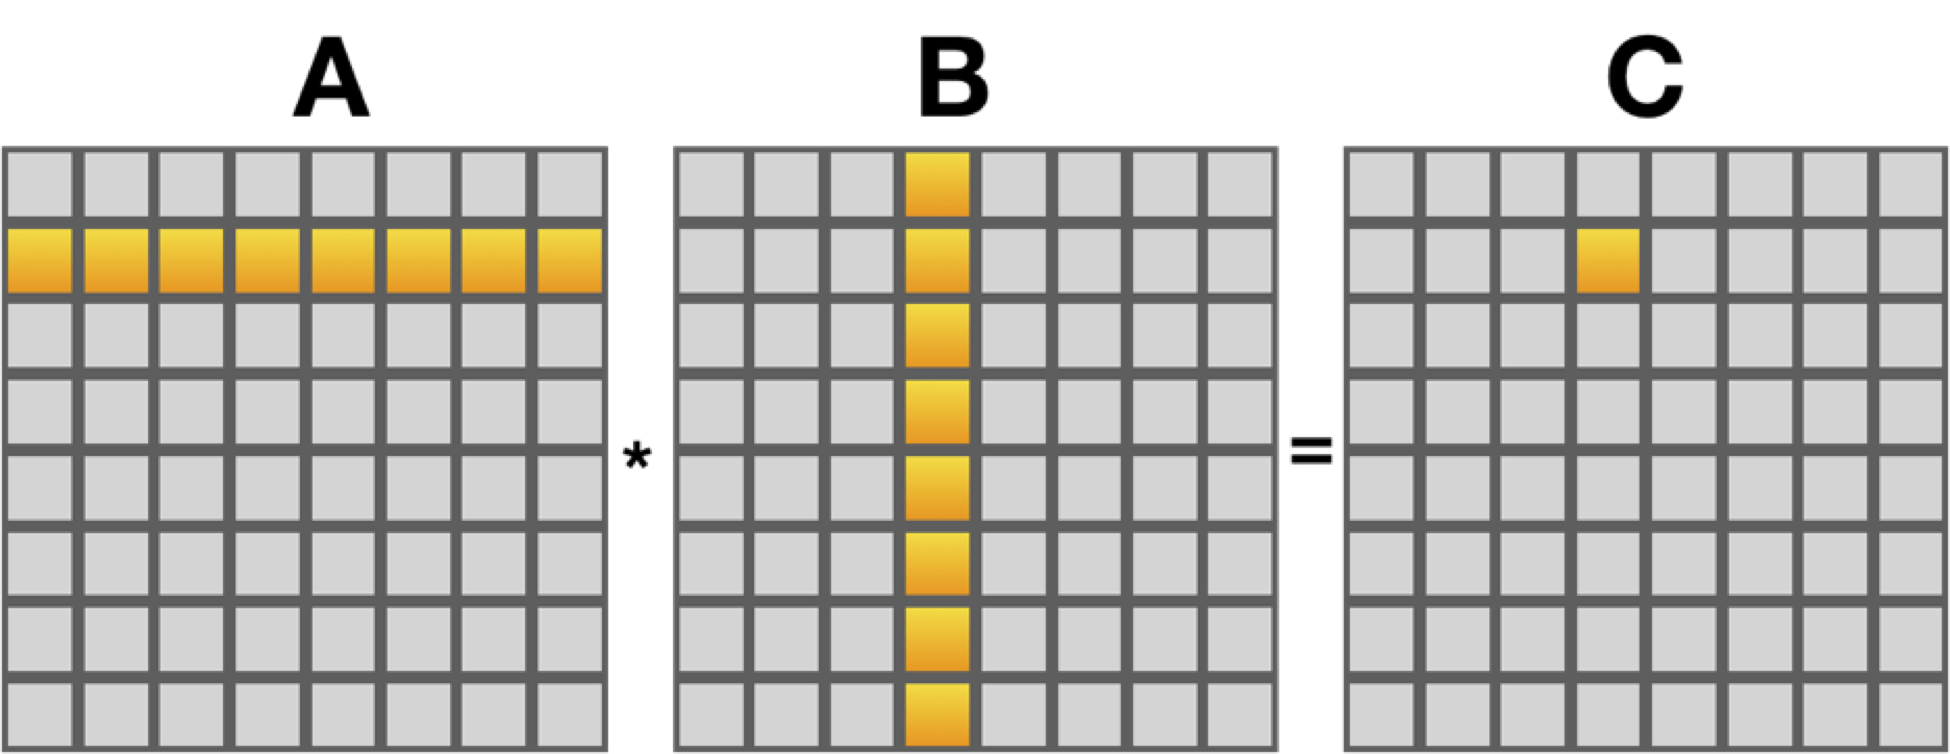
\includegraphics{matmul_naive.png}
\end{figure}

这一矩阵乘法的算法复杂度是$O(n^3)$的。而这一实现实际是非常没有效率的。现代CPU 是普遍具备 SIMD (单指令多数据)支持的,同时在很多的计算指令中,乘法和加法是支持聚合为一个乘累加操作的,即 Multiply and 
Acculturation 或者 FMA(fused multiply-add)。而在方法\ref{code:matmul_naive} 中实现的矩阵乘法实际上是受到内存限制的,从而不能充分利用CPU 的计算能力。而通过SIMD 可以单次处理多个数据的能力,处理器
每次从主内存中(main memory )中加载一个缓存行(cache line )到 L1 高速缓存中,而此后CPU 每次计算则可以从cache line中加载单个数据。尽管这种处理并不理想,但是矩阵B 中处理的情形则更加低效。处理矩阵 B
的过程中,由于矩阵的数据排布(data layout)在这里是 row major 的, 即内存中二维矩阵B 中最内层的储存上相邻的数据实际上是同一行的,的在沿着矩阵的列方向加载 B 中的一个 cache line之后,实际只使用了其中
的一个元素而已,cache line 中包含的是处于同一行的多列元素的值,这些加载到的元素中除了第一个元素被使用到了,其他元素均被浪费。
而在扫描完了B 中整整这一列的数据之后,开始扫描B 的下一列数据时,处理器则早已刷新了缓存。

在矩阵乘法优化中的一种可行的策略是优化 B 中的 memory efficiency,比较直观的一种想法是每次计算中使用从矩阵 B 中加载的 cache line 中的多个元素。将矩阵 A 中的加载的值同矩阵B中加载的多个连续值相乘。而
另外一方面,矩阵乘法有一个属性在于:矩阵 A 乘 矩阵 B 实际上是将矩阵A 中的列以矩阵 B 中的列元素作为参数的线性组合,或者说是,矩阵 B 中的行已矩阵 A 中的行元素作为参数的线性组合。

首先,矩阵的右乘,可以视作列的组合;对于简单的矩阵右乘一个列向量的情形

\begin{equation}
  \begin{pmatrix}
    x_1 & y_1 & z_1\\
    x_2 & y_2 & z_2\\  
    x_3 & y_3 & z_3
  \end{pmatrix}
  \times 
  \begin{pmatrix}
    a \\
    b \\
    c
  \end{pmatrix}
  = 
  \begin{pmatrix}
    ax_1 + by_1 + cz_1\\
    ax_2 + by_2 + cz_2\\  
    ax_3 + by_3 + cz_3
  \end{pmatrix}
\end{equation}

而对于这一过程做一个直观的可视化可以表示为

\begin{figure}
  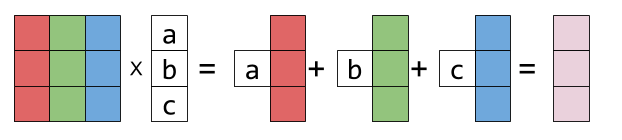
\includegraphics{matvec.png}
\end{figure}

矩阵中的每一列同列向量中的每个元素相乘,矩阵中的一列同列向量中的单个元素(Scalar)的乘积仍是一个列向量,而最终的结果则是这些列向量的和。
这一情形推广到右乘一个矩阵则是相似的情形,乘积的结果的矩阵中的每一列仍是矩阵列的线性组合。

\begin{equation}
  \begin{pmatrix}
    x_1 & y_1 & z_1\\
    x_2 & y_2 & z_2\\  
    x_3 & y_3 & z_3
  \end{pmatrix}
  \times 
  \begin{pmatrix}
    a & d & g\\
    b & e & h\\
    c & f & i
  \end{pmatrix}
  = 
  \begin{pmatrix}
    ax_1 + by_1 + cz_1 & dx_1 + ey_1 + fz_1 & gx_1 + hy_1 + iz_1 \\
    ax_2 + by_2 + cz_2 & dx_2 + ey_2 + fz_2 & gx_2 + hy_2 + iz_2 \\
    ax_3 + by_3 + cz_3 & dx_3 + ey_3 + fz_3 & gx_3 + hy_3 + iz_3
  \end{pmatrix}
\end{equation}

这一过程的可视化表示如下图所示

\begin{figure}
  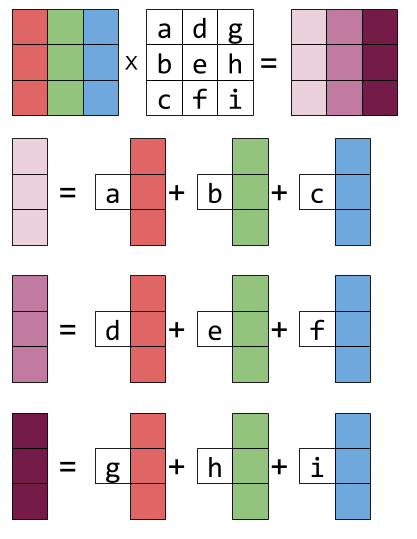
\includegraphics{matmul_right.png}
\end{figure}

而对于左乘一个矩阵则可以视为是矩阵行的线性组合。首先对于一个矩阵左乘一个行向量的情形,可以表示为

\begin{equation}
  \begin{pmatrix}
    a & b & c
  \end{pmatrix}
  \times
  \begin{pmatrix}
    x_1 & y_1 & z_1 \\
    x_2 & y_2 & z_2 \\
    x_3 & y_3 & z_3 
  \end{pmatrix}
  = 
  \begin{pmatrix}
    ax_1 + bx_2 + cx_3 & ay_1 + by_2 + cy_3 & az_1 + bz_2 + cz_3
  \end{pmatrix}
\end{equation}
可视化表示为

\begin{figure}
  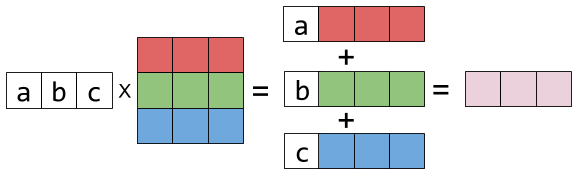
\includegraphics{vecmat.png}
\end{figure}

而在左乘一个矩阵的过程中,则是左乘行向量的情形重复作用于矩阵中的每一行。相对应的可视化表示可以为

\begin{figure}
  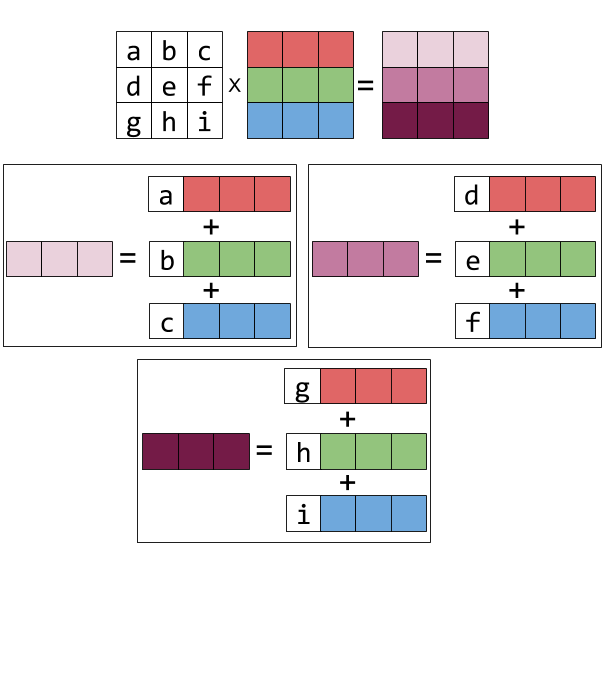
\includegraphics{matmul_left.png}
\end{figure}

于是考虑到矩阵B 的缓存性能的优化策略在于,可以从矩阵A中加载一个元素,并将其广播填满SIMD 寄存器,而矩阵B 中的连续元素也被加载到对应的
SIMD 寄存器,因此两者可以实现元素间乘法的矢量计算,实际上,很多硬件的指令中是支持按照矢量寄存器的 data lane 进行计算的,完全可以
加载A 中的多个元素到矢量寄存器 R,再以R 中的data lane 实现A中的单个值(Scalar)同B 中加载的多个元素的乘法,而将
单个元素广播填满单个SIMD 矢量寄存器的操作,在存在这一支持的情况下大可不必,同时很可以实现寄存器的节约和运算成本的降低。

这一优化策略使得参与计算的矩阵B 的存储带宽(memory bandwidth)获得了较为充分的利用,而换个角度来看硬件资源的利用,现代CPU 一般存在
多个用于调度分配SIMD 计算的执行端口,和多个用于调度数据存取的端口。这意味着,在一个时钟周期里可以实现调度执行多条读取数据的指令,或者
调度执行多条乘法计算指令。在硬件水平上,处理器中的寄存器间的操作的速度是远远高于缓存的读写性能,而缓存的读写性能又远远高于内存,内存的
读写性能则又远远高于硬盘等外部存储,高性能计计算的过程中对于存储性能的优化的目标在于尽可能的减小访问存储的操作同计算操作的比例,提高
高速设备中数据的利用率,在算法的设计上保证加载到高速设备上的数据得到充分利用,并可复用。而在实现矩阵乘法的背景下,这就意味着,从矩阵 A 中
加载的数据需要被用来执行多次计算操作,这一点可以由上述方法中,A 中的元素同来自B 中的同一 cache line 中不同列的元素做计算而保证;同时,
B 中的元素也需要被用于执行不止一次计算,而要实现这一点,则可以通过加载数据时,从矩阵 A 中每次加载多行的元素,从而使得B 中的每一列的元素
可以得到复用。而从计算结果来看,乘积矩阵 C 中的每一行的元素都是一个矢量累加值,每次处理多行A 中的元素的效应则是,矩阵 C 中处理中需要多个
寄存器来存储这些矢量累加值,从使用一个寄存器到使用一块(patch/block)寄存器因此这一过程。因此,这一过程被称为寄存器 blocking (register blocking)

\begin{figure}
  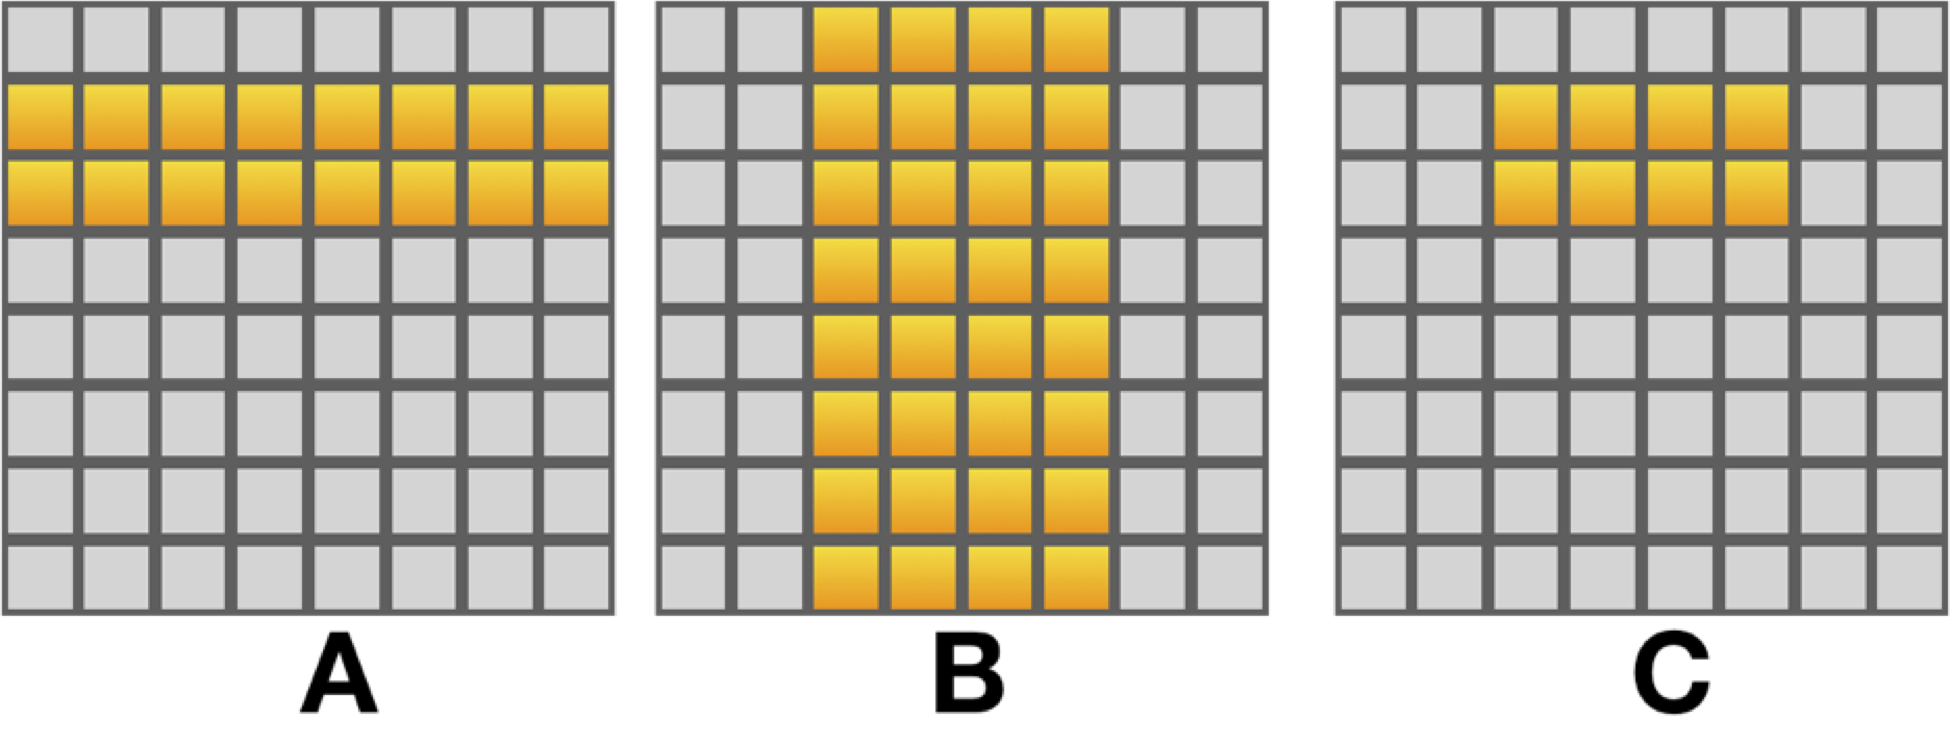
\includegraphics{zregblock.png}
\end{figure}

尽管上述的实现已经让计算中的内存访问机制(memory access pattern)变得相对有效,但是仍然具有着优化的空间。在顺序计算矩阵 C 中的一行中连续
的元素时,需要多次访问呢矩阵 B,加载矩阵B 中不同行的元素,而这一过程中,B 中的值会同时加载到缓存中,由于用于计算的寄存器和缓存都是有限的,
而且一般容量都很小, 这意味着按照这样的顺序访问 B 矩阵,必然 会使得B 的缓存失效。

计算矩阵C 中的一个子矩阵的顺序会影响到矩阵A 和矩阵 B 的内存访问模式。理想的内存访问模式是 将矩阵B加载到我们的L1缓存中,并保存很长时间 。
实现此目的的一种方法是对矩阵C的计算进行分块。而在每次计算中只需要计算 C 中被分割出的这一块即可。对应的伪码实现如下:

\begin{listing}
  \label{code:tiled_matmul}
  for i = 1 to N
    for j = 1 to N
      { read block C{i,j} to fast memory }
      for k = 1 to N
        {read block A{i, k} to fast memory}
        {read block B{k, j} to fast memory}
        
        C{i, j} = A{i, k} * B{k, j} // matrix multiplication on tile
      { write C{i, j} to slow memory }
\end{listing}

假设A, B, C 矩阵都是 $n x n$ 的矩阵,这里对于矩阵的分块每一个小块的尺度则是 $b x b$,记 $N = n / b$ , 这一算法在低速存储设备上的存储访问操作(memory operation)
为

\begin{align}
  NUMBER_MEM_OPS = N \times n^2 // read each block of B N^3 times (N^3 \times \frac{n}{N} \times \frac{n}{N} )
                 + N \times n^2 // read each block of A N^3
                 + 2 \times n^2 // read and write of block C
                 = (2\times N + 2)n^2
\end{align}

于是在这一算法实现下的矩阵乘法中,计算操作同访存操作的比值为 $2\times N^3 / ((2\times N + 2)n^2) \approx n / N = b$,
在 n 足够大是,这一近似成立。因而可以通过矩阵分块计算中的block size块大小实现这一算法的效率提升,同时block size也并不是可以任意大,
这一优化的出发点在于优化利用快速缓存,而这一值同时也受到缓存大小的限制,上述矩阵乘法中的三个块 $A{i, k}, B{k, j}, C{i, j} $ 均必须
不能溢出快速缓存的容量限制,

总结而言,充分考虑到硬件环境的高效矩阵乘法的实现如图所示:

在如下图所示的矩阵乘法算法中。首先,将大小为m,n和k的矩阵乘法在 k 所表示的维度以$k_c$ 大小的高速缓存块进行分割,从而创建rank为k的子问题。 在这一阶段,
为了实现在计算的最基础层次上上,参与计算的元素在存储中是完全连续的,即矩阵表示中最低维度对应的stride为unit stride,需要将B以一种特殊的格式分块打包到连续存储中
(标记为\bar{B})。 然后,将每个rank为k的子问题沿m维度,按照缓存块大小$m_c$分块,从而创建block-panel子问题。 然后将当前的$m_c×k_c$块, 记为$A_i$, 按照计算中的
最基础级别,参与计算的元素在存储中是连续的的原则,打包到\bar{A}。 然后将剩下的该block-panel子问题($C_i:= C_i + \bar{A}_i \bar{B}$)实现为高度优化的汇编
计算内核。 而该内核将继续沿$n$,$m_c$划分矩阵,最后在$k_c$维划分矩阵。

\begin{figure}
  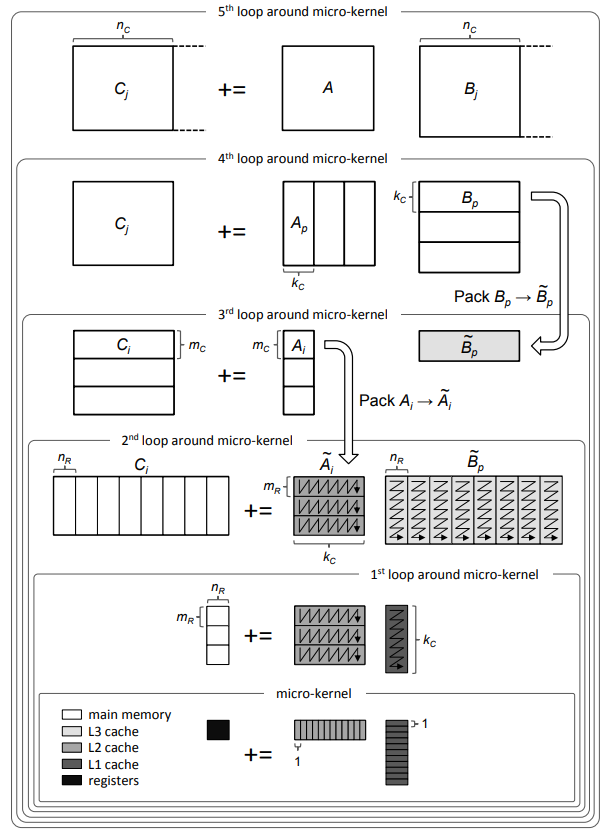
\includegraphics{gemm.png}
\end{figure}

这一矩阵乘法中的多个循环的使用在于根据缓存块大小和寄存器的容量,精心设计矩阵的分块策略,从而使得子矩阵的分布同存储的层级结构相匹配,以达到数据复用的目的。
同时A 和B 的子矩阵被复制打包到临时工作区(workspace),从而使得矩阵乘法操作的micro-kernel能够在内存中连续访问矩阵元素,从而提高了缓存和TLB性能。而一般
打包过程的成本可以通过计算本身来摊销,在计算的规模足够大时,这一成本是可以忽略不记的。

而这其中决定最内层的循环的调用的寄存器相关的参数 $m_r$, $n_r$, 以及较外层的循环调用的高速缓存相关参数 $m_c$, $k_c$, $n_c$ 一般由具体硬件的特性所决定,
比如矢量寄存器的大小,缓存大小,缓存的相关性等。Analytical Modeling Is Enough for High-Performance BLIS 为这些参数的选择提供了一种分析性模型。

\section{FFT 卷积实现同Winograd 卷积的对比}

\subsection{FFT快速卷积实现概述}
对于信号处理中的场景而言,频域中的乘法对应于时域中的卷积。 使用DFT将输入信号转换到频域,再乘以滤波器的频率响应,然后使用Inverse DFT将输入信号转换回时域。
从傅立叶时代开始这种基本技术就广为人知。 但是,因为计算DFT所需的时间比直接计算卷积所需的时间长,所以使用傅里叶变换实现卷积的方法并没有受到足够的重视。
随着1965年快速傅立叶变换(FFT)的发展,这种情况发生了变化。 通过使用FFT算法计算DFT,与直接对时域信号进行卷积相比,通过频域进行卷积可以更快。而卷积的运算量
则获得了有效的缩减。

基于FFT的卷积方法可以表示为

\begin{align}
  f * g = F^{-1}(F(f)  \cdot F(g))
\end{align}
其中的$F$ 与 $F^{-1}$ 表示傅里叶变换和逆傅里叶变换,在离散场景下,$f$ 和 $g$ 需要具有相同数目的元素,这一点可以通过向两者中较短的那一方实现 zero padding实现。
DFT卷积的结果是一个循环卷积(circular convolution/ cyclic convolution),而从中获得有效的卷积结果仍然需要从循环卷积的结果中抽取其中的最后 $|f| - |g| + 1 $
个元素。

\subsection{FFT卷积与Winograd卷积}
离散傅里叶变换方法的有效卷积可以视作 Winograd 卷积 \ref{eq:winograd1d} 的一种特殊情形,其中的矩阵$AT^$, $B^T$ 和 $G$ 均处于复数域,并且由多项式点
( polynomial point)为单位根的范德蒙矩阵(Vandermonde matrices)推导出。

Winograd 与 FFT 卷积中主要能够降低计算成本的一点在于,权重的变换可以预先计算,而卷积输入的变换则可以多次复用,而计算本身中比重最大的部分仍然是矩阵乘法

在FFT 方法的卷积实现中,需要计算表示图像/特征块(feature map tile)的变换值和权重的变换值的复数张量之间的接口乘法。这一过程也支持变换后的Tensor 的多次复用。
在执行图像块的变换后,产生一个复数张量 $U = U_r + U_i$ ,可以计算实值张量 $U_r + U_i$ 并将其与Ur和Ui一起存储。 类似地,张量 $V_i - V_r$ 和 $V_r + V_i$
 可以在内核变换期间计算, 并与 $V_r$ 一起存储(不必存储$V_i$ )。 然后,可以用三个独立的实值张量的元素间乘积替换复数张量的元素间乘积. 而由此计算得到的三个
 实数张量则可以在计算逆变换的过程中被隐式的转换为单个实数张量。总体来讲,快速复数乘法的实现,可以使得原本的复数域中的一个矩阵间乘法转换为3个实数域中的矩阵乘法,
 同直接计算复数乘法相比,可以将乘法的操作数减少 25\%.

另外一方面,实数域中的信号的 FFT 变换是具有 Hermitian 对称性(Hermitian symmetry)的, 即实数矩阵在傅里叶变换之后的矩阵同其共轭转置矩阵(conjugate transpose)是相等的,
这使得在 FFT 卷积方法中的矩阵乘法部分的实际有效乘法量可以进一步减半。一个尺寸为 $m x m$ 的实数值矩阵的离散傅里叶变换由于 Hermitian 对称性可以用 $ m x (floor(\frac{1}{2} + 1)) $ 
个复数来表示。同时又由于 $ U^H V^H = ( UV )^H $,矩阵乘法结果中的一半元素的值(上/下三角)可以通过取已计算值的共轭获得。

\subsection{图片分块方法实现}
在信号处理中,在很多场景下,需要处理的信号都非常长,计算过程中往往没有足够的内存可以容纳需要处理的整段输入。而另外一方面,由于卷积本身是
线性的,因此可以通过简单的将输入的每个输出块相加来计算长序列信号的输出。因此可以通过 overlap-add方法实现长序列的分割,从而将长序列分解成为更易于处理的段序列。
而对于卷积网络中所使用的对于filter 尺寸为 r 且输出为 m 的卷积,通过OLA(overlap-add)方法,卷积的输入被分割为 $m + r - 1$的小块,而块之间存在着 $r-1$ 的重叠(overlap)。而对于
所有输入图像中相同位置的图块,计算输出图像大小为m的图块

\subsection{复数乘法计算}
复数计算在信号处理中有着广泛的应用,然而不幸的是,很多现代硬件在底层的指令上则缺少直接计算复数计算的支持,这使得复数计算的实现不得不面临着额外的挑战和付出。
而针对于ARM平台,尽管在ARMv8.2指令集(ISA) 之后添加了 FCADD (Floating-point Complex Add), FCMLA (Floating-point Complex Multiply Accumulate) 操作,
然而实现这一指令集的芯片微架构(microarchitecture)并不占据主流,主要集中在高端智能收集芯片上,比如苹果应用于iPhone X上的A11芯片及其之后的应用于iPhone XS系列的
A12芯片以及iPhone 11 的 A13芯片,在很多的嵌入式设备场景下的low profile的计算资源场景下,指令级别的复数操作支持仍然是缺失的。

一般的复数乘法中,一对复数相乘需要四次复数乘法,即

\begin{align}
\label{eq:complex_mul}
  (u_r + i u_i) (v_r + i v_i) = u_r v_r - u_i v_i + i ( u_i v_r + u_r v_i )
\end{align}

而对于\ref{eq:complex_nul} 稍加变换既可以得到复数乘法的快速算法,该方法只需要三个实数乘法。

\begin{align}
\label{eq:complex_mul_fast}
  (u_r + i u_i) (v_r + i v_i) &= [ u_r v_r - u_i v_i, i(u_r v_i + u_i v_r)]
                               &= [ u_a - u_c,i( u_a + u_b) ]
\end{align}

where 
\begin{align}
u_a = v_r ( u_r + u_i )
u_b = u_r ( v_i - v_r )
u_c = u_i ( v_r + v_i )
\end{align}

这一方法,通过使用更多的加法实现对于乘法的减少 

\section{F(4x4, 3x3, 6x6) 的实现}

最为常用的 F(4, 3) Winograd 卷积中的权重变换矩阵为

\begin{align}
  G = 
  \begin{pmatrix}
    \frac{1}{4} & 0 & 0 \\
    -\frac{1}{6} & -\frac{1}{6} & -\frac{1}{6} \\
    -\frac{1}{6} & \frac{1}{6} & -\frac{1}{6} \\
    \frac{1}{24} & \frac{1}{12} & \frac{1}{6} \\
    \frac{1}{24} & -\frac{1}{12} & \frac{1}{6} \\
    0 & 0 & 1
  \end{pmatrix}
\end{align}

将这个变换矩阵转变为整数矩阵需要对其乘24,而对于变换矩阵扩大24倍,将会对于计算带来相当的额外开销。
在执行Winograd 变换时,空间域的权重需要至少额外增加 $floor(\log_{2}{24^2}) = 10$ 位来表示其数值
以免数值溢出。此时如果输入的权重类型为8 位整数,则经过Winograd 变换之后,其数值表示则不得不由32位
整数作表示。

而如果考虑到Winograd变换在复数域中可能的取值,则这一问题存在着相对较为简单的表示。尽管在复数域导出
Winograd 算法的动机看似是有点不合理的,毕竟在前文中也提到了Winograd 卷积同基于DFT 的卷积实现的联系,
以及Winograd 卷积相对DFT卷积的优势。Winograd 卷积从效果上来看,可以看作全实数表示的DFT卷积,Winograd
卷积在卷积尺度较小的场景下相对于DFT卷积的优势也正是来自于实数乘法的复杂度低于复数乘法。因此,在Winograd
算法中引入复数,看上去是一个在效率上有所倒退的举动。但实际上,这里的出发点在于获得更加简单的变换矩阵
表示,从而在引入可接受的运算开销的前提下实现量化计算。

\begin{align}

B^T = 
\begin{pmatrix}
  1 & 0 & 0 & 0 -1 & 0 \\
  0 & 1 & 1 & 1 & 1 & 0\\
  0 & -1 & 1 & -1 & 1 & 0 \\
  0 & -i & -1 & i & 1 & 0 \\
  0 & i & -1 & -i & 1 & 0 \\
  0 & -1 & 0 & 0 & 0 & 1
\end{pmatrix}

G = 
\begin{pmatrix}
  1 & 0 & 0 \\
  \frac{1}{4} & \frac{1}{4} & \frac{1}{4} \\
  \frac{1}{4} & -\frac{1}{4} & \frac{1}{4} \\
  \frac{1}{4} & \frac{i}{4} & -\frac{1}{4} \\
  \frac{1}{4} & -\frac{i}{4} & -\frac{1}{4} \\
  0 & 0 & 1 \\
\end{pmatrix}

A^T = 
\begin{pmatrix}
  1 & 1 & 1 & 1 &1 &0\\ 
  0 & 1 & −1 & i & −i & 0\\
  0 & 1 & 1 & −1 & −1 & 0\\
  0 & 1 & −1 & −i & i & 1
\end{pmatrix}

\end{align}
% !TeX root = ../main.tex

\chapter{卷积操作实现优化}
\label{cha:chapter04}

\section{线程并行化}
前面描述的方法对于计算的并行化处理大多处于指令级别,通过SIMD 矢量处理器的数据并行化处理,
实现指令级别的并行化(Instruction Level Parallelism, ILP)。除此之外,多线程
执行也是实现并行计算的重要手段,称为线程级并行化(Thread Level Parallelism, TLP)。
线程级的并行化处理可以对于处理器内核(core)的计算资源的更为有效的利用,多线程的处理可以
使得superscalar\footnote{超标量体系结构是许多处理器中使用的并行计算方法。 在超标量计算机中,中央处理单元(CPU)管理多个指令流水线,以在一个时钟周期内同时执行多个指令。 这是通过将不同的流水线通过处理器中的多个执行单元来实现的。 为了成功实现超标量架构,CPU的指令获取机制必须智能地检索和委托指令。 否则,可能会发生管道停顿,从而导致执行单元经常处于空闲状态。
} 架构的处理器的执行单元被全部调用,同时通过流水线(pipeline)调度来隐藏
访存所需要的延时(memory latency)。而使用线程并行化的同时也存在着一些额外的需求或者
开销: 首先需要额外的存储满足线程上下文(thread context)的需求,而线程并行化也要求被
优化的程序具有在最基础的指令并行之外的并行度;另外一方面,多线程也会对于内存带宽带来额外的
压力,更多的线程,意味着每个单独的线程所获得的缓存空间会更小。

当前的绝大多数的基于ARM 架构的SoC 都会集成多个 CPU core, 另外ARM 也在计算密集的场景下针对性
的对于处理器添加了SMT(Simultaneous multithreading )支持,比如针对于自动驾驶应用优化的Cortex 
A76AE 微架构。

在实现计算的多线程并行化的过程中,不仅仅要保证被并行的任务中的子任务之间没有依赖,保证子任务
执行的独立性,同时需要避免在多线程执行中可能存在的 False Sharing 和 Cache Line Ping-pong.

\begin{itemize}
  \item 当不同的线程具有程序中未共享的数据,但此数据被映射到共享的缓存行(cache line)时,
  就会发生False Sharing。 例如,假设一个程序具有一个整数数组,其中一个线程执行读取和写
  入具有偶数索引的所有数组条目,而另一个线程执行读取和写入具有奇数索引的条目。 在这种情况下
  ,线程实际上将不会共享数据,但是它们将共享高速缓存行,因为每条高速缓存行都将包含奇数和偶数
  索引值。
  \item 高速缓存行ping-pong是在多个CPU(或内核)之间快速连续传输高速缓存行的效果。
  本质上,如果多个CPU试图在同一高速缓存行中读取和写入数据,则该高速缓存行可能必须快速连续地
  在两个线程之间传输,并且这可能会导致性能显着下降(甚至与单线程相比,性能可能更差)。
\end{itemize}

针对于此,实现多线程处理中需要特别注意以下几点:

\begin{itemize}
    \item 尽可能向同一个CPU 执行写入操作;
    \item 为每个CPU 指定对应的内存;将线程锁定在对应的CPU;
    \item 避免将频繁读写但本身并没有关联的数据放在同一个 Cache Line 中;
\end{itemize}

因此在实现过程中,这里结合本文中的 Winograd 卷积实现设计的空间局部区域的独立性,在特征的输入
变换,GEMM 实现,以及结果的输出变换中,对于整体的图像或者中间特征做了区域性的划分,并在这一层级
上实现多线程的并行,保证每个单独的region 的处理都是独立的,并且向各个处理阶段对应的buffer 输出
处理结果的过程中,各个region 所对应的地址空间避开处于同一cache line的情形。从而保证这一 regional wise
的 Winograd 算法实现在多线程并行下的高效性。


\seciont{端到端整数计算支持}

在量化计算的量化策略中,本文选择了一种相对简单有效且在实际平台可以具有广泛应用和实现的方案。

矩阵中的每个值均以放射变换的方法(线性变换)通过比例因子和零点值被量化映射到低精度的表示,因此量化域(这里的实现为
8为无符号整数)中的计算可以
直接映射到实数域。比例因子和零点值被矩阵中的多个值所共享,即矩阵中的所有行使用相同的比例因此和零点。
量化矩阵中的值 $x_r$可以通过如下简单的变换方式实现到实数矩阵中的值 $x_q$ 的变换。

\begin{align}
  x_r = a_{scale} (x_q - a_{zero_point})
\end{align}

这里的比例因子(scale factor) $a_scale$ 一般而言是一个浮点值,而参考在 \cite{Jacob2017QuantizationAT}
对于比例因此的处理,按照上面的实数域和量化域的表示,实数域的值 $x_r, y_r, z_r$ 所对应的量化域中的值分别为
$x_q, y_q, z_q$,三者各自对应的比例因子为 $x_{scale}, y_{scale}, z_{scale}$ , 零点为 $x_{zero}, y_{zero},
 z_{zero}$
那么对应的实数域的乘法的计算可以表示为

\begin{align}
\label{eq:quan_arith}
z_r &= x_r \cdot y_r
z_{scale} \cdot (z_q - z_{zero}) &= (x_{scale} \cdot (x_q - x_{zero})) \cdot (y_{scale} \cdot (y_q - y_{zero}))
z_q - z_{zero} &= \frac{x_{scale}\cdot y_{scale}}{z_{scale}} (x_q - x_{zero}) (y_q - y_{zero})
z_q &= \frac{x_{scale}\cdot y_{scale}}{z_{scale}} (x_q - x_{zero}) (y_q - y_{zero}) + z_{zero}
\end{align}

这里\ref{eq:quan_arith} 可见实数乘法所对应的量化值乘法,也具备着同实数值和量化值的映射所类似的线性变换形式,
而这里的比例因子 $ M = \frac{x_{scale} y_{scale}}{z_{scale}}$, 按照 \cite{Jacob2017QuantizationAT} 中的经验性
统计可以表示为
\begin{align}
M = 2^{-n} M_0
\end{align}
而其中, $M_0 \in [0.5, 1)$ 且 n 为非负整数。$ M_0$现在很适合表示为定点乘法器(例如,int16或int32取决于硬件)。
例如,如果使用int32,则表示$M_0$的整数是最接近$2^{31}M_0$的int32值。 由于$M_0> 0.5$,因此该值始终至少为$2^{30}$,
因此始终至少具有30位相对精度。 因此,与$M_0$的乘法可以实现为定点乘法。 同时乘以$2^{-n}$可以有效移位来实现

另外,这里的实现中计算操作的输入和网络的权重均为8位无符号整数表示,8位整数的乘法一般会使用32位的累加器,
而在Winograd 卷积实现的将输入由空间域向winograd域 变换过程中,F(2,3) 的Winograd 算法中基本只涉及加减操作,
在这一过程中将输入的无符号8位整数转换为16位带符号整数做处理,并且在后续的矩阵乘法操作中实现中使用 32 位的累加器,
每次乘累加操作中,将16位整数乘法的结果widen 到32位再加到32位的累加器中。而在一般的基于GEMM的量化卷积实现中,
累加结束后,会再次通过量化,将32位 的整数表示转换位8位整数的表示,这一过程可以称为再量化(re-quantization )或者后累加量化(post-accumulation quantization)
而Winograd 卷积的实现中,乘累加操作结束之后,还需要执行输出变换操作,将Winograd 域中的矩阵乘法结果转换回空间域,
此后再执行量化,并将量化之后的8位整数输出,从而降低对于内存带宽的压力和缓存占用。

\section{卷积相关操作的融合}

此外,现在通用的卷积网络中,卷积操作之后通常还带有bias,而在卷积操作之后还通常会紧随着Batch Normalization 操作
和 Relu 激活函数,这一流程构成了卷积网络中常用的一大范式即,Conv(+ Bias)-> BatchNorm -> Relu。相比于卷积操作
而言添加Bias,并对输出的特征作Batch Normalization 和 relu激活本身从计算复杂度角度而言,都是不值一提的,但是在
ARM 设备的这种嵌入市场景下,将这几个流程作为单独的操作在模型的运行时顺序执行,则是需要额外的存储消耗的(memory 
footprint)。每次执行单个操作的过程中,都需要从memory系统中读入上一操作输出的特征,并且把简单计算操作之后的结果
再写入memory,这同在嵌入式场景计算和存储资源受限的条件下需要最大化计算/访存操作的比例的优化目标是相悖的。而注意到
这些后续的操作实际上都是可以转化为区域性(regional wise)inplace 的操作的,特别是Batch Normalization 在模型训练
结束之后,单纯作inference的过程中是可以和卷积操作实现融合的。以下简述Batch Normalization 同卷积的融合的过程。

对于Batch Norm 的输入特征 $x$, Batch Norm 本身的参数 $\gamma$, $\beta$, 以及训练过程中对于输入特征的统计量
(exponential moving average)$\mu$ $\sigma$. 操作对应的输出则为 $\tilde{x}$,Batch Norm 操作的形式如下:

\begin{align}
\label{eq:bn}
\tilde{x_i} = \gamma \frac{x_i - \mu}{\sqrt{\sigma^2 + \epsilon}} + \beta
\end{align}

而这一操作可以通过 1x1 卷积实现。给定一个输入特征 F,其data layout 为 $C \times H \times W$, 其对应的Batch Norm的
结果$\hat{F}$可通过计算每个空间位置$i, j$的如下矩阵-矢量乘法获得:

\begin{align}
\label{eq:bn_matvec}
\begin{pmatrix}
\hat{F_{1,i,j}} \\
\hat{F_{2,i,j}} \\
\vdots \\
\hat{F_{C,i,j}}
\end{pmatrix}
=
\begin{pmatrix}
\frac{\gamma_{1}{\sqrt{\sigma_{1}^2 + \epsilon}}} & 0 & \dots & 0 \\
0 & \frac{\gamma_{2}{\sqrt{\sigma_{2}^2 + \epsilon}}}  & \dots & 0 \\
\vdots \\
0 & 0 & \dots & \frac{\gamma_{C}{\sqrt{\sigma_{C}^2 + \epsilon}}} 
\end{pmatrix}
+
\begin{pmatrix}
\begin{pmatrix}
F_{1,i,j} \\
F_{2,i,j} \\
\vdots \\
F_{C,i,j}
\end{pmatrix}
+ 
\begin{pmatrix}
\beta_{1} - \gamma_1 \frac{\mu_1}{\sqrt{\sigma_1^2 + \epsilon}}\\
\beta_{2} - \gamma_2 \frac{\mu_2}{\sqrt{\sigma_2^2 + \epsilon}}\\
\vdots\\
\beta_{C} - \gamma_C \frac{\mu_C}{\sqrt{\sigma_C^2 + \epsilon}}\\
\end{pmatrix}
\end{align}

而Batch Norm操作往往又紧随卷积操作,于是可以将Batch Norm操作融合入卷积操作,将上述的batch norm的矩阵表示\label{eq:bn_matvec}
表示为 $\hat{F} = W_{bn} \cdot F + b_{bn}$, 其中 $W_{bn} \in R^{CxC}, b_{bn} \in R^C$, 而嵌入Batch Norm 
操作前继的卷积操作之后,这一计算过程则为:
\begin{align}
\hat{f_{i,j}} = W_{bn} \cdot (W_{conv} \cdot f_{i,j} + b_{conv}) + b_{bn}
\end{align}

于是卷积和Batch Norm 两个操作可以通过一个权重为 $W = W_{bn} \cdot W_{conv}$, Bias 为 $b = W_{bn} \cdot b_{conv} + b_{bn}$
的卷积操作来替代。

除此之外,对卷积的添加Bias 和relu激活,则可以在Winograd卷积的每个子区域的输出变换过程中,在重量化之前,
in-place的实现添加Bias,而在重量化之后,通过输出值截断(output clamping),实现诸如 Relu或者 Relu6 这样
的简单的激活函数,从而减少模型运行时对于内存的开销。

\section{NEON 计算指令优化}

到目前实现为止,在ARM 处理器上最为广泛得以应用的并行计算资源便是NEON,这一技术自ARMv7-A ISA起成为ARM芯片
的处理计算密集型应用的最为通用的主力解决方案,而ARM 也在ARM v8.2A指令架构中提出了对于NEON的矢量计算的扩展
SVE(Scalable Vector Extension),然而作为一项可选的扩展,目前的通用ARM计算设备中几乎没有支持这一特性(富士通
的下一代超算使用ARM架构,支持SVE)。另外例如高通这样的集成电路设计者会在SoC方案中添加一些专门的计算单元,比如
高通的Hexagon DSP针对性的优化了对于量化计算的支持,HTA(Hexagon Tensor Accelerator), HVX(Hexagon Vector 
eXtension) 的支持,使得在这种设备上的on device 模型推理计算有了额外的优化途径,并减轻了CPU的压力。同时NVIDIA
也为其面向移动端的ARM 架构芯片提供了GPU 和Cuda 支持。但是这些额外的专门硬件的支持网络模型推理计算的方案,局限性
也是显而易见的,即受到硬件本身的局限,不具备通用性。在实现可移植,强适应性,高效率的计算密集应用下,NEON还是
目前最优的选择。

在细节上实现高效的NEON指令的调用以及调度对于在ARM 架构设备上的高效智能计算具有着至关重要的意义。在实现量化的
快速卷积过程中,本作遵循了以下优化原则:

\begin{itemize}
    \item 连续的计算指令之间不得存在数据依赖。某些计算指令,比如乘累加,的操作延时(latency)比较高, 为了减少指令等待时间,
    需要避免将当前指令的目标寄存器用作下一条指令的源寄存器。在实现中,这里将 vld(数据加载), vmlal(乘累加),st(数据写出)
    等操作在调度的过程中实现第一阶段通过多个vld 指令加载各项所需的数据,第二阶段 通过乘累加操作计算相互独立的矢量计算,这里
    每个乘累加操作需要有各自独立的累加器,否则累加过程会存在data dependence 造成指令stall。第三 阶段再将乘累加的结果写出。
    \item NEON/FPU是一个独立的处理单元,Load/Store Unit也是一个独立处理单元,两个单元可以并行执行。Load/Store Unit可以在
    加载到第一个数据的时候立即把数据forward给NEON/FPU,这样在只有一条VLDM指令时,只需要引入1个CPU cycles的延迟了。
    这就提示我们通过合理的打散VLDM指令并和NEON/FPU指令交织(interleave),可以提升指令执行的并行度,并继 续提升软件的性能。
    \item NEON指令执行计算的过程中不得出现条件分支。NEON指令集中没有分支跳转指令。 当需要跳转时,使用ARM的跳转指令。 在ARM
    处理器中,分支预测技术被广泛使用。 但是一旦分支预测失败,那么惩罚就会很高。 因此,最好避免使用跳转说明。
\end{itemize}

\section{Winograd 算法数值稳定性}

尽管Winograd 算法是现已知的在计算复杂度而言最优的卷积算法, 然而 Winograd 卷积算法具有着数值
计算不稳定的特质。在卷积的尺度相对比较小(比如F(2,3), F(4, 3)),并且参与运算的数值为单精度或
者双精度浮点数时,Winograd 卷积的结果仍然是相当精确的,但是当卷积的尺度变大,或者参数计算的数值
精度降低时,这一情况却不容乐观了。这也限制了Winograd 卷积的适用范围,在卷积核或者卷积操作输入的
子块的尺度较大的情形下,Winograd卷积的精确性便会有比较明显的损失。 Winograd 卷积计算的精确性
可以通过找出更加合适的Winograd 算法的导出式有关,即通过 Toom-Cook 算法或者CRP理论选择合适的
interpolation points导出对应的输入变化,权重变换和输出变换矩阵。 这里需要说明的一点是,Winograd 
卷积的数值不稳定性,带来的只是一种边际数值误差(marginal error),因此,Winograd 卷积在很多情形
下只是应用于模型 的推理阶段,
即网络在训练的过程中使用常规的卷积算法,而在模型前向推理的过程中,是完全可以将对应的满足条件的
卷积操作可以替换为 Winograd 卷积算法。

\begin{table}[]
\label{tbl:winograd_acc}
\caption{ResNet 18 在不同尺度和不同精度的Winograd 卷积算法下的CIFAR-10 分类准确率}
\begin{tabular}{llll}
\hline
\multicolumn{1}{|l|}{}                 & \multicolumn{1}{l|}{32 bit} & \multicolumn{1}{l|}{16 bit} & \multicolumn{1}{l|}{8 bit} \\ \hline
\multicolumn{1}{|l|}{Direct  Conv}     & \multicolumn{1}{l|}{93.16}  & \multicolumn{1}{l|}{93.60}  & \multicolumn{1}{l|}{93.22} \\ \hline
\multicolumn{1}{|l|}{Winograd F(2, 3)} & \multicolumn{1}{l|}{93.16}  & \multicolumn{1}{l|}{93.48}  & \multicolumn{1}{l|}{93.21} \\ \hline
\multicolumn{1}{|l|}{Winograd F(4, 3)} & \multicolumn{1}{l|}{93.14}  & \multicolumn{1}{l|}{19.25}  & \multicolumn{1}{l|}{17.36} \\ \hline
Winograd F(6, 3)                       & 93.11                       & 11.41                       & 10.95                     
\end{tabular}
\end{table}

表 \ref{tbl:winograd_acc} 中对比了不同尺度的Winograd 卷积算法在不同精度的数据表示下的准确度及数值
稳定性,这里以直接卷积算法的准确率作为对照,可见对于输出尺度大于2 的 Winograd 卷积在low precision 
的场景下在对应视觉任务上的准确率会大幅下降,而这里指的Winograd 卷积指的是在 \cite{Lavin2015FastAF}
以及附带的Toom Cook 方法代码中所导出Winograd 算法形式。究其原因在于,在Winograd 卷积的输出尺度较大
时, 如\ref{eq:winograd_f43} 可见,在变换矩阵 $A^T, G, B^T$ 中对应的数值的范围会变大,并且注意,在
卷积神经网络中常用的2D 卷积中,将其转换为整数型计算时,权重变换矩阵 G 需要扩大 24 倍,则卷积计算过程
中,至少要保证在 $\pm24^2$ 范围内数据的表示和计算数值精度 。
\begin{align}
\label{eq:winograd_f43}
  A^T = 
  \begin{pmatrix}
      1 & 1 & 1 &  1 &  1 &  0\\
      0 & 1 & -1&  2 &  -2&  0\\
      0 & 1 & 1 &  4 &  4 &  0\\
      0 & 1 & -1&  8 &  -8&  1
  \end{pmatrix}
  G = 
  \begin{pmatrix}
    \frac{1}{4} & 0 & 0 \\
    -\frac{1}{6} & -\frac{1}{6} & -\frac{1}{6} \\
    -\frac{1}{6} & \frac{1}{6} & -\frac{1}{6} \\
    \frac{1}{24} & \frac{1}{12} & \frac{1}{6} \\
    \frac{1}{24} & -\frac{1}{12} & \frac{1}{6} \\
    0 & 0 & 1
  \end{pmatrix}
  B^T =
  \begin{pmatrix}
    4  & 0 &  -5 & 0  &  1&  0\\
    0  & -4&  -4 & 1  &  1&  0\\
    0  & 4 &  -4 & -1 &  1&  0\\
    0  & -2&  -1 & 2  &  1&  0\\
    0  & 2 &  -1 & -2 &  1&  0\\
    0  & 4 &  0  & -5 &  0&  1
  \end{pmatrix}
\end{align}

\section{实验验证}

这一部分验证本文中实现的整数Winograd 快速卷积在嵌入式设别上的有效性,
包括
\begin{itemize}
  \item 针对单个卷积操作本身的执行效率,测量不同尺度规模的卷积输入下
    \begin{itemize}
        \item 该卷积实现同对应的全精度Winograd快速卷积的加速效果, 包括执行效率和内存开销(对照组为NNPACK实现)
        \item 该卷积实现同基于GEMM卷积方法的整数卷积效率对比(对照组为QNNPACK实现)
    \end{itemize}
  \item 针对于由此卷积操作构成的卷积网络在特定的视觉任务上的的执行性能和效率
    \begin{itemize}
        \item 同全精度网络的执行效率和准确率作对比加速效果存储开销和数值精度
        \item 同支持量化卷积计算的模型推理框架(TensorFlow lite, PyTorch Mobile)对比实现的准确率与加速效果
    \end{itemize}

\end{itemize}
\chapter{总结与展望}

\section{论文工作总结}

本文主要研究整数型Winograd 卷积在ARM CPU上的高效实现,从而加速卷积神经网络在ARM上的运行效率。对于
智能应用在移动和边缘设备的部署具备着积极的意义。

移动设备上运行卷积网络当前最大的痛点在于卷积网络庞大的计算量与移动设备有限的计算能力之间的矛盾。
而同时,尽管模型量化方法已经存在了众多研究,但在支持量化网络模型在移动设备上的高效执行方面,业界
依然存在着相当的空白。本文针对上述的难点和痛点,将目前已经的计算复杂度最低的卷积算法针对ARM 设备
硬件特性,实现改造调整,并且结合线性量化策略,实现卷积网络中端到端的整数计算流程。对比于现有的移动端
框架对于卷积网络的实现,取得了相对的效率提升。以下是本文完成的主要工作内容:

\begin{itemize}
    \item Winograd 算法可以在广泛存在移动端和边缘计算设备上的ARM CPU上实现计算复杂度的降低和计算功耗的节省。
    Winograd 卷积运行的过程中有着输入变换和输出变换带来的额外开销,Winograd 卷积主要是加速效果来自于减少了
    乘法操作,因而这二者带来的开销需要通过GEMM计算来做摊销。
    所以在Winograd卷积的运行中可见,卷积的输出通道数越大,卷积的加速效果越明显越接近于Winograd卷积加速的理论值。
    文中针对于Arm Cortex A设备,通过空间局部区域多通道处理方法,高效的使用ARMv8-A NEON SIMD 指令,
    实现了移动/嵌入式场景下内存有限, 计算能力受限的状态下,Winograd 卷积的高效实现。
    对每个卷积输出的子区域,独立并行计算这一多通道区域的输入变换, 矩阵乘法和输出变换。输入变换的
    16个空间位置的结果 被scatter到16 组Winograd域中的GEMM计算中,之后并行执行这16组GEMM,即输入变换
    和权重变换的结果的乘积,最后从对应的16组GEMM中 gather 到每个区域对应的结果,执行输出变换,将
    最后的结果变换回空间域的值并作输出。并且在data layout,权重预处理,中间结果存储(store)等等方面
    为此算法的实现和ARM Cortex A架构的特征做了设计。 
    \item 结合上面的整数卷积方法实现,本文应用静态线性量化策略,使用整数模拟逼近浮点数计算,
    实现了在网络中的端到端完全的整数计算。通过引入位移和和加法操作,使得量化模型中的整数值计算同
    全精度模型中的实数计算相对应。而且引入的额外操作的复杂度相对于网络本身的计算而言可以忽略不记。
    最后考虑到卷积网络在移动端的实现,并在卷积的操作中实现了batch norm,relu,bias等操作的融合,
    并入,尽可能减少在存储和计算上不必要的开销,实现卷积网络在移动端CPU的执行效率。
\end{itemize}

\section{未来工作展望}

本文实现了针对于移动端 ARM 设备的整数型Winograd 快速卷积。一定程度上提高了移动端卷积网络的运行
效率。但是,目前的工作仍然有着相当的提升空间。

\begin{itemize}
    \item 本文中优化的Winograd 卷积算法为Winograd卷积算法中尺度较小的 F(2,3) 卷积,该算法
    理论上的加速上限为2.25倍。而Winograd 算法会随着卷积尺度的增大而加速效果更加明显,同时,其
    数值精度也会下降,而在模型参数的数值精度比较低的场景下,即量化网络的场景下,在卷积规模变大
    时,计算的数值稳定性和精度会大幅下降。这里一项重要的原因在于没有找到在卷积尺度变大的场景下
    适合与低精度计算的Winograd算法的形式,即对应的三个变换矩阵。目前主流使用的Winograd 变换
    中的数值的范围在卷积尺度变大时明显变大,而量化网络中数值的范围包括中间特征的范围则是非常有限的。
    所以完全发挥出Winograd卷积在量化场景下的加速效果,还需要找到数值范围相对较小的 Winograd变换
    的形式,克服这一场景下Winograd卷积的数值不稳定性。
    \item 目前的实现中计算的主要负载由NEON实现,但在众多的ARM设备中除了CPU中的SIMD协处理器可以
    用于实现并行计算,很多设备同时还具有GPU支持,而对于移动设备中种类繁多的GPU存在着统一可移植
    的通用接口 - Vulkan。在ARM 设备上使用Vulkan API 在GPU上执行神经网络模型的推理计算将更有效
    的实现,同时更充分的利用设备硬件资源。
\end{itemize}


% 其它部分
\backmatter

%% 本科生要求的几个索引。
% \listoffigures    % 插图索引
% \listoftables     % 表格索引
% \listofequations  % 公式索引

% 参考文献
\bibliographystyle{thuthesis-numeric}      % 顺序编码制
% \bibliographystyle{thuthesis-author-year}  % 著者-出版年制
% \bibliographystyle{thuthesis-bachelor}     % 本科生参考文献的著录格式
\bibliography{ref/refs}

% 致谢
% !TeX root = ../main.tex

\begin{acknowledgements}
  衷心感谢导师 xxx 教授和物理系 xxx 副教授对本人的精心指导。他们的言传身教将使
  我终生受益。

  在美国麻省理工学院化学系进行九个月的合作研究期间,承蒙 xxx 教授热心指导与帮助,不
  胜感激。感谢 xx 实验室主任 xx 教授,以及实验室全体老师和同学们的热情帮助和支
  持!本课题承蒙国家自然科学基金资助,特此致谢。

  感谢 \LaTeX{} 和 \thuthesis\cite{thuthesis},帮我节省了不少时间。
\end{acknowledgements}


% 声明
\statement

% 附录
% \appendix
% % !TeX root = ../main.tex

\begin{survey}
\label{cha:survey}

\title{Title of the Survey}
\maketitle

写出至少 5000 外文印刷字符的调研阅读报告或者书面翻译 1-2 篇(不少于 2 万外文印刷符)。

It is impossible to cover in a single chapter every concept of mathematical
programming.\cite{tex} This chapter introduces only the basic concepts and techniques of
mathematical programming such that readers gain an understanding of them
throughout the book\cite{abrahams99tex,salomon1995advanced}.


\section{Single-Objective Programming}
The general form of single-objective programming (SOP) is written
as follows,
\begin{equation*} % 如果附录中的公式不想让它出现在公式索引中,那就请
                             % 用 equation*
\left\{\begin{array}{l}
\max \,\,f(x)\\[0.1 cm]
\mbox{subject to:} \\ [0.1 cm]
\qquad g_j(x)\le 0,\quad j=1,2,\cdots,p
\end{array}\right.
\end{equation*}
which maximizes a real-valued function $f$ of
$x=(x_1,x_2,\cdots,x_n)$ subject to a set of constraints.

\newcommand\Real{\mathbf{R}}
\newtheorem{mpdef}{Definition}[chapter]
\begin{mpdef}
In SOP, we call $x$ a decision vector, and
$x_1,x_2,\cdots,x_n$ decision variables. The function
$f$ is called the objective function. The set
\begin{equation*}
S=\left\{x\in\Real^n\bigm|g_j(x)\le 0,\,j=1,2,\cdots,p\right\}
\end{equation*}
is called the feasible set. An element $x$ in $S$ is called a
feasible solution.
\end{mpdef}

\newtheorem{mpdefop}[mpdef]{Definition}
\begin{mpdefop}
A feasible solution $x^*$ is called the optimal
solution of SOP if and only if
\begin{equation}
f(x^*)\ge f(x)
\end{equation}
for any feasible solution $x$.
\end{mpdefop}

One of the outstanding contributions to mathematical programming was known as
the Kuhn-Tucker conditions\ref{eq:ktc}. In order to introduce them, let us give
some definitions. An inequality constraint $g_j(x)\le 0$ is said to be active at
a point $x^*$ if $g_j(x^*)=0$. A point $x^*$ satisfying $g_j(x^*)\le 0$ is said
to be regular if the gradient vectors $\nabla g_j(x)$ of all active constraints
are linearly independent.

Let $x^*$ be a regular point of the constraints of SOP and assume that all the
functions $f(x)$ and $g_j(x),j=1,2,\cdots,p$ are differentiable. If $x^*$ is a
local optimal solution, then there exist Lagrange multipliers
$\lambda_j,j=1,2,\cdots,p$ such that the following Kuhn-Tucker conditions hold,
\begin{equation}
\label{eq:ktc}
\left\{\begin{array}{l}
    \nabla f(x^*)-\sum\limits_{j=1}^p\lambda_j\nabla g_j(x^*)=0\\[0.3cm]
    \lambda_jg_j(x^*)=0,\quad j=1,2,\cdots,p\\[0.2cm]
    \lambda_j\ge 0,\quad j=1,2,\cdots,p.
\end{array}\right.
\end{equation}
If all the functions $f(x)$ and $g_j(x),j=1,2,\cdots,p$ are convex and
differentiable, and the point $x^*$ satisfies the Kuhn-Tucker conditions
(\ref{eq:ktc}), then it has been proved that the point $x^*$ is a global optimal
solution of SOP.

\subsection{Linear Programming}
\label{sec:lp}

If the functions $f(x),g_j(x),j=1,2,\cdots,p$ are all linear, then SOP is called
a {\em linear programming}.

The feasible set of linear is always convex. A point $x$ is called an extreme
point of convex set $S$ if $x\in S$ and $x$ cannot be expressed as a convex
combination of two points in $S$. It has been shown that the optimal solution to
linear programming corresponds to an extreme point of its feasible set provided
that the feasible set $S$ is bounded. This fact is the basis of the {\em simplex
  algorithm} which was developed by Dantzig as a very efficient method for
solving linear programming.
\begin{table}[ht]
\centering
  \centering
  \caption*{Table~1\hskip1em This is an example for manually numbered table, which
    would not appear in the list of tables}
  \label{tab:badtabular2}
  \begin{tabular}[c]{|m{1.5cm}|c|c|c|c|c|c|}\hline
    \multicolumn{2}{|c|}{Network Topology} & \# of nodes &
    \multicolumn{3}{c|}{\# of clients} & Server \\\hline
    GT-ITM & Waxman Transit-Stub & 600 &
    \multirow{2}{2em}{2\%}&
    \multirow{2}{2em}{10\%}&
    \multirow{2}{2em}{50\%}&
    \multirow{2}{1.2in}{Max. Connectivity}\\\cline{1-3}
    \multicolumn{2}{|c|}{Inet-2.1} & 6000 & & & &\\\hline
    \multirow{2}{1.5cm}{Xue} & Rui  & Ni &\multicolumn{4}{c|}{\multirow{2}*{\thuthesis}}\\\cline{2-3}
    & \multicolumn{2}{c|}{ABCDEF} &\multicolumn{4}{c|}{} \\\hline
\end{tabular}
\end{table}

Roughly speaking, the simplex algorithm examines only the extreme points of the
feasible set, rather than all feasible points. At first, the simplex algorithm
selects an extreme point as the initial point. The successive extreme point is
selected so as to improve the objective function value. The procedure is
repeated until no improvement in objective function value can be made. The last
extreme point is the optimal solution.

\subsection{Nonlinear Programming}

If at least one of the functions $f(x),g_j(x),j=1,2,\cdots,p$ is nonlinear, then
SOP is called a {\em nonlinear programming}.

A large number of classical optimization methods have been developed to treat
special-structural nonlinear programming based on the mathematical theory
concerned with analyzing the structure of problems.
\begin{figure}[h]
  \centering
  
\includegraphics{thu-lib-logo.pdf}
  \caption*{Figure~1\quad This is an example for manually numbered figure,
    which would not appear in the list of figures}
  \label{tab:badfigure2}
\end{figure}

Now we consider a nonlinear programming which is confronted solely with
maximizing a real-valued function with domain $\Real^n$.  Whether derivatives are
available or not, the usual strategy is first to select a point in $\Real^n$ which
is thought to be the most likely place where the maximum exists. If there is no
information available on which to base such a selection, a point is chosen at
random. From this first point an attempt is made to construct a sequence of
points, each of which yields an improved objective function value over its
predecessor. The next point to be added to the sequence is chosen by analyzing
the behavior of the function at the previous points. This construction continues
until some termination criterion is met. Methods based upon this strategy are
called {\em ascent methods}, which can be classified as {\em direct methods},
{\em gradient methods}, and {\em Hessian methods} according to the information
about the behavior of objective function $f$. Direct methods require only that
the function can be evaluated at each point. Gradient methods require the
evaluation of first derivatives of $f$. Hessian methods require the evaluation
of second derivatives. In fact, there is no superior method for all
problems. The efficiency of a method is very much dependent upon the objective
function.

\subsection{Integer Programming}

{\em Integer programming} is a special mathematical programming in which all of
the variables are assumed to be only integer values. When there are not only
integer variables but also conventional continuous variables, we call it {\em
  mixed integer programming}. If all the variables are assumed either 0 or 1,
then the problem is termed a {\em zero-one programming}. Although integer
programming can be solved by an {\em exhaustive enumeration} theoretically, it
is impractical to solve realistically sized integer programming problems. The
most successful algorithm so far found to solve integer programming is called
the {\em branch-and-bound enumeration} developed by Balas (1965) and Dakin
(1965). The other technique to integer programming is the {\em cutting plane
  method} developed by Gomory (1959).

\hfill\textit{Uncertain Programming\/}\quad(\textsl{BaoDing Liu, 2006.2})

\bibliographystyle{plainnat}
\bibliography{ref/refs,ref/appendix}

\end{survey}
       % 本科生:外文资料的调研阅读报告
% % !TeX root = ../main.tex

\begin{translation}
\label{cha:translation}

\title{书面翻译题目}
\maketitle

\section{单目标规划}
北冥有鱼,其名为鲲。鲲之大,不知其几千里也。化而为鸟,其名为鹏。鹏之背,不知其几
千里也。怒而飞,其翼若垂天之云。是鸟也,海运则将徙于南冥。南冥者,天池也。
\begin{equation}\tag*{(123)}
 p(y|\mathbf{x}) = \frac{p(\mathbf{x},y)}{p(\mathbf{x})}=
\frac{p(\mathbf{x}|y)p(y)}{p(\mathbf{x})}
\end{equation}

吾生也有涯,而知也无涯。以有涯随无涯,殆已!已而为知者,殆而已矣!为善无近名,为
恶无近刑,缘督以为经,可以保身,可以全生,可以养亲,可以尽年。

\subsection{线性规划}
庖丁为文惠君解牛,手之所触,肩之所倚,足之所履,膝之所倚,砉然响然,奏刀騞然,莫
不中音,合于桑林之舞,乃中经首之会。
\begin{table}[ht]
\centering
  \centering
  \caption*{表~1\hskip1em 这是手动编号但不出现在索引中的一个表格例子}
  \label{tab:badtabular3}
  \begin{tabular}[c]{|m{1.5cm}|c|c|c|c|c|c|}\hline
    \multicolumn{2}{|c|}{Network Topology} & \# of nodes &
    \multicolumn{3}{c|}{\# of clients} & Server \\\hline
    GT-ITM & Waxman Transit-Stub & 600 &
    \multirow{2}{2em}{2\%}&
    \multirow{2}{2em}{10\%}&
    \multirow{2}{2em}{50\%}&
    \multirow{2}{1.2in}{Max. Connectivity}\\\cline{1-3}
    \multicolumn{2}{|c|}{Inet-2.1} & 6000 & & & &\\\hline
    \multirow{2}{1.5cm}{Xue} & Rui  & Ni &\multicolumn{4}{c|}{\multirow{2}*{\thuthesis}}\\\cline{2-3}
    & \multicolumn{2}{c|}{ABCDEF} &\multicolumn{4}{c|}{} \\\hline
\end{tabular}
\end{table}

文惠君曰:“嘻,善哉!技盖至此乎?”庖丁释刀对曰:“臣之所好者道也,进乎技矣。始臣之
解牛之时,所见无非全牛者;三年之后,未尝见全牛也;方今之时,臣以神遇而不以目视,
官知止而神欲行。依乎天理,批大郤,导大窾,因其固然。技经肯綮之未尝,而况大坬乎!
良庖岁更刀,割也;族庖月更刀,折也;今臣之刀十九年矣,所解数千牛矣,而刀刃若新发
于硎。彼节者有间而刀刃者无厚,以无厚入有间,恢恢乎其于游刃必有余地矣。是以十九年
而刀刃若新发于硎。虽然,每至于族,吾见其难为,怵然为戒,视为止,行为迟,动刀甚微,
謋然已解,如土委地。提刀而立,为之而四顾,为之踌躇满志,善刀而藏之。”

文惠君曰:“善哉!吾闻庖丁之言,得养生焉。”


\subsection{非线性规划}
孔子与柳下季为友,柳下季之弟名曰盗跖。盗跖从卒九千人,横行天下,侵暴诸侯。穴室枢
户,驱人牛马,取人妇女。贪得忘亲,不顾父母兄弟,不祭先祖。所过之邑,大国守城,小
国入保,万民苦之。孔子谓柳下季曰:“夫为人父者,必能诏其子;为人兄者,必能教其弟。
若父不能诏其子,兄不能教其弟,则无贵父子兄弟之亲矣。今先生,世之才士也,弟为盗
跖,为天下害,而弗能教也,丘窃为先生羞之。丘请为先生往说之。”
\begin{figure}[h]
  \centering
  
\includegraphics{thu-whole-logo.pdf}
  \caption*{图~1\hskip1em 这是手动编号但不出现索引中的图片的例子}
  \label{tab:badfigure3}
\end{figure}

柳下季曰:“先生言为人父者必能诏其子,为人兄者必能教其弟,若子不听父之诏,弟不受
兄之教,虽今先生之辩,将奈之何哉?且跖之为人也,心如涌泉,意如飘风,强足以距敌,
辩足以饰非。顺其心则喜,逆其心则怒,易辱人以言。先生必无往。”

孔子不听,颜回为驭,子贡为右,往见盗跖。

\subsection{整数规划}
盗跖乃方休卒徒大山之阳,脍人肝而餔之。孔子下车而前,见谒者曰:“鲁人孔丘,闻将军
高义,敬再拜谒者。”谒者入通。盗跖闻之大怒,目如明星,发上指冠,曰:“此夫鲁国之
巧伪人孔丘非邪?为我告之:尔作言造语,妄称文、武,冠枝木之冠,带死牛之胁,多辞缪
说,不耕而食,不织而衣,摇唇鼓舌,擅生是非,以迷天下之主,使天下学士不反其本,妄
作孝弟,而侥幸于封侯富贵者也。子之罪大极重,疾走归!不然,我将以子肝益昼餔之膳。”


\nocite{abrahams99tex,salomon1995advanced}
\bibliographystyle{plainnat}
\bibliography{ref/appendix}

% 也可以使用 thebiliography 环境手写
% \begin{thebibliography}{2}
%   \bibitem{abrahams99tex}
%   P.~W. Abrahams, K.~Berry, and K.~A. Hargreaves, \emph{{\TeX} for the
%     Impatient}.\hskip 1em plus 0.5em minus 0.4em\relax Addison-Wesley, 1990.

%   \bibitem{salomon1995advanced}
%   D.~Salomon, ``The advanced {\TeX}book.''\hskip 1em plus 0.5em minus 0.4em\relax
%     New York: Springer, 1995.
% \end{thebibliography}


\end{translation}
  % 本科生:外文资料的书面翻译
% \chapter{单目标规划}

As one of the most widely used techniques in operations
research, \emph{ mathematical programming} is defined as a means of maximizing a
quantity known as \emph{bjective function}, subject to a set of constraints
represented by equations and inequalities. Some known subtopics of mathematical
programming are linear programming, nonlinear programming, multiobjective
programming, goal programming, dynamic programming, and multilevel
programming.

It is impossible to cover in a single chapter every concept of mathematical
programming. This chapter introduces only the basic concepts and techniques of
mathematical programming such that readers gain an understanding of them
throughout the book.


\section{Single-Objective Programming}
The general form of single-objective programming (SOP) is written
as follows,
\begin{equation*} % 如果附录中的公式不想让它出现在公式索引中,那就请
                             % 用 equation*
\left\{\begin{array}{l}
\max \,\,f(x)\\[0.1 cm]
\mbox{subject to:} \\ [0.1 cm]
\qquad g_j(x)\le 0,\quad j=1,2,\cdots,p
\end{array}\right.
\end{equation*}
which maximizes a real-valued function $f$ of
$x=(x_1,x_2,\cdots,x_n)$ subject to a set of constraints.

\newcommand\Real{\mathbf{R}}
\newtheorem{mpdef}{Definition}[chapter]
\begin{mpdef}
In SOP, we call $x$ a decision vector, and
$x_1,x_2,\cdots,x_n$ decision variables. The function
$f$ is called the objective function. The set
\begin{equation*}
S=\left\{x\in\Real^n\bigm|g_j(x)\le 0,\,j=1,2,\cdots,p\right\}
\end{equation*}
is called the feasible set. An element $x$ in $S$ is called a
feasible solution.
\end{mpdef}

\newtheorem{mpdefop}[mpdef]{Definition}
\begin{mpdefop}
A feasible solution $x^*$ is called the optimal
solution of SOP if and only if
\begin{equation}
f(x^*)\ge f(x)
\end{equation}
for any feasible solution $x$.
\end{mpdefop}

One of the outstanding contributions to mathematical programming was known as
the Kuhn-Tucker conditions\ref{eq:ktc}. In order to introduce them, let us give
some definitions. An inequality constraint $g_j(x)\le 0$ is said to be active at
a point $x^*$ if $g_j(x^*)=0$. A point $x^*$ satisfying $g_j(x^*)\le 0$ is said
to be regular if the gradient vectors $\nabla g_j(x)$ of all active constraints
are linearly independent.

Let $x^*$ be a regular point of the constraints of SOP and assume that all the
functions $f(x)$ and $g_j(x),j=1,2,\cdots,p$ are differentiable. If $x^*$ is a
local optimal solution, then there exist Lagrange multipliers
$\lambda_j,j=1,2,\cdots,p$ such that the following Kuhn-Tucker conditions hold,
\begin{equation}
\label{eq:ktc}
\left\{\begin{array}{l}
    \nabla f(x^*)-\sum\limits_{j=1}^p\lambda_j\nabla g_j(x^*)=0\\[0.3cm]
    \lambda_jg_j(x^*)=0,\quad j=1,2,\cdots,p\\[0.2cm]
    \lambda_j\ge 0,\quad j=1,2,\cdots,p.
\end{array}\right.
\end{equation}
If all the functions $f(x)$ and $g_j(x),j=1,2,\cdots,p$ are convex and
differentiable, and the point $x^*$ satisfies the Kuhn-Tucker conditions
(\ref{eq:ktc}), then it has been proved that the point $x^*$ is a global optimal
solution of SOP.

\subsection{Linear Programming}
\label{sec:lp}

If the functions $f(x),g_j(x),j=1,2,\cdots,p$ are all linear, then SOP is called
a {\em linear programming}.

The feasible set of linear is always convex. A point $x$ is called an extreme
point of convex set $S$ if $x\in S$ and $x$ cannot be expressed as a convex
combination of two points in $S$. It has been shown that the optimal solution to
linear programming corresponds to an extreme point of its feasible set provided
that the feasible set $S$ is bounded. This fact is the basis of the {\em simplex
  algorithm} which was developed by Dantzig as a very efficient method for
solving linear programming.
\begin{table}[ht]
\centering
  \centering
  \caption*{Table~1\hskip1em This is an example for manually numbered table, which
    would not appear in the list of tables}
  \label{tab:badtabular2}
  \begin{tabular}[c]{|m{1.5cm}|c|c|c|c|c|c|}\hline
    \multicolumn{2}{|c|}{Network Topology} & \# of nodes &
    \multicolumn{3}{c|}{\# of clients} & Server \\\hline
    GT-ITM & Waxman Transit-Stub & 600 &
    \multirow{2}{2em}{2\%}&
    \multirow{2}{2em}{10\%}&
    \multirow{2}{2em}{50\%}&
    \multirow{2}{1.2in}{Max. Connectivity}\\\cline{1-3}
    \multicolumn{2}{|c|}{Inet-2.1} & 6000 & & & &\\\hline
    \multirow{2}{1.5cm}{Xue} & Rui  & Ni &\multicolumn{4}{c|}{\multirow{2}*{\thuthesis}}\\\cline{2-3}
    & \multicolumn{2}{c|}{ABCDEF} &\multicolumn{4}{c|}{} \\\hline
\end{tabular}
\end{table}

Roughly speaking, the simplex algorithm examines only the extreme points of the
feasible set, rather than all feasible points. At first, the simplex algorithm
selects an extreme point as the initial point. The successive extreme point is
selected so as to improve the objective function value. The procedure is
repeated until no improvement in objective function value can be made. The last
extreme point is the optimal solution.

\subsection{Nonlinear Programming}

If at least one of the functions $f(x),g_j(x),j=1,2,\cdots,p$ is nonlinear, then
SOP is called a {\em nonlinear programming}.

A large number of classical optimization methods have been developed to treat
special-structural nonlinear programming based on the mathematical theory
concerned with analyzing the structure of problems.
\begin{figure}[h]
  \centering
  
\includegraphics{thu-lib-logo.pdf}
  \caption*{Figure~1\quad This is an example for manually numbered figure,
    which would not appear in the list of figures}
  \label{tab:badfigure2}
\end{figure}

Now we consider a nonlinear programming which is confronted solely with
maximizing a real-valued function with domain $\Real^n$.  Whether derivatives are
available or not, the usual strategy is first to select a point in $\Real^n$ which
is thought to be the most likely place where the maximum exists. If there is no
information available on which to base such a selection, a point is chosen at
random. From this first point an attempt is made to construct a sequence of
points, each of which yields an improved objective function value over its
predecessor. The next point to be added to the sequence is chosen by analyzing
the behavior of the function at the previous points. This construction continues
until some termination criterion is met. Methods based upon this strategy are
called {\em ascent methods}, which can be classified as {\em direct methods},
{\em gradient methods}, and {\em Hessian methods} according to the information
about the behavior of objective function $f$. Direct methods require only that
the function can be evaluated at each point. Gradient methods require the
evaluation of first derivatives of $f$. Hessian methods require the evaluation
of second derivatives. In fact, there is no superior method for all
problems. The efficiency of a method is very much dependent upon the objective
function.

\subsection{Integer Programming}

{\em Integer programming} is a special mathematical programming in which all of
the variables are assumed to be only integer values. When there are not only
integer variables but also conventional continuous variables, we call it {\em
  mixed integer programming}. If all the variables are assumed either 0 or 1,
then the problem is termed a {\em zero-one programming}. Although integer
programming can be solved by an {\em exhaustive enumeration} theoretically, it
is impractical to solve realistically sized integer programming problems. The
most successful algorithm so far found to solve integer programming is called
the {\em branch-and-bound enumeration} developed by Balas (1965) and Dakin
(1965). The other technique to integer programming is the {\em cutting plane
  method} developed by Gomory (1959).

\hfill\textit{Uncertain Programming\/}\quad(\textsl{BaoDing Liu, 2006.2})

\section{单目标规划}
北冥有鱼,其名为鲲。鲲之大,不知其几千里也。化而为鸟,其名为鹏。鹏之背,不知其几
千里也。怒而飞,其翼若垂天之云。是鸟也,海运则将徙于南冥。南冥者,天池也。
\begin{equation}\tag*{(123)}
 p(y|\mathbf{x}) = \frac{p(\mathbf{x},y)}{p(\mathbf{x})}=
\frac{p(\mathbf{x}|y)p(y)}{p(\mathbf{x})}
\end{equation}

吾生也有涯,而知也无涯。以有涯随无涯,殆已!已而为知者,殆而已矣!为善无近名,为
恶无近刑,缘督以为经,可以保身,可以全生,可以养亲,可以尽年。

\subsection{线性规划}
庖丁为文惠君解牛,手之所触,肩之所倚,足之所履,膝之所倚,砉然响然,奏刀騞然,莫
不中音,合于桑林之舞,乃中经首之会。
\begin{table}[ht]
\centering
  \centering
  \caption*{表~1\hskip1em 这是手动编号但不出现在索引中的一个表格例子}
  \label{tab:badtabular3}
  \begin{tabular}[c]{|m{1.5cm}|c|c|c|c|c|c|}\hline
    \multicolumn{2}{|c|}{Network Topology} & \# of nodes &
    \multicolumn{3}{c|}{\# of clients} & Server \\\hline
    GT-ITM & Waxman Transit-Stub & 600 &
    \multirow{2}{2em}{2\%}&
    \multirow{2}{2em}{10\%}&
    \multirow{2}{2em}{50\%}&
    \multirow{2}{1.2in}{Max. Connectivity}\\\cline{1-3}
    \multicolumn{2}{|c|}{Inet-2.1} & 6000 & & & &\\\hline
    \multirow{2}{1.5cm}{Xue} & Rui  & Ni &\multicolumn{4}{c|}{\multirow{2}*{\thuthesis}}\\\cline{2-3}
    & \multicolumn{2}{c|}{ABCDEF} &\multicolumn{4}{c|}{} \\\hline
\end{tabular}
\end{table}

文惠君曰:“嘻,善哉!技盖至此乎?”庖丁释刀对曰:“臣之所好者道也,进乎技矣。始臣之
解牛之时,所见无非全牛者;三年之后,未尝见全牛也;方今之时,臣以神遇而不以目视,
官知止而神欲行。依乎天理,批大郤,导大窾,因其固然。技经肯綮之未尝,而况大坬乎!
良庖岁更刀,割也;族庖月更刀,折也;今臣之刀十九年矣,所解数千牛矣,而刀刃若新发
于硎。彼节者有间而刀刃者无厚,以无厚入有间,恢恢乎其于游刃必有余地矣。是以十九年
而刀刃若新发于硎。虽然,每至于族,吾见其难为,怵然为戒,视为止,行为迟,动刀甚微,
謋然已解,如土委地。提刀而立,为之而四顾,为之踌躇满志,善刀而藏之。”

文惠君曰:“善哉!吾闻庖丁之言,得养生焉。”


\subsection{非线性规划}
孔子与柳下季为友,柳下季之弟名曰盗跖。盗跖从卒九千人,横行天下,侵暴诸侯。穴室枢
户,驱人牛马,取人妇女。贪得忘亲,不顾父母兄弟,不祭先祖。所过之邑,大国守城,小
国入保,万民苦之。孔子谓柳下季曰:“夫为人父者,必能诏其子;为人兄者,必能教其弟。
若父不能诏其子,兄不能教其弟,则无贵父子兄弟之亲矣。今先生,世之才士也,弟为盗
跖,为天下害,而弗能教也,丘窃为先生羞之。丘请为先生往说之。”
\begin{figure}[h]
  \centering
  
\includegraphics{thu-whole-logo.pdf}
  \caption*{图~1\hskip1em 这是手动编号但不出现索引中的图片的例子}
  \label{tab:badfigure3}
\end{figure}

柳下季曰:“先生言为人父者必能诏其子,为人兄者必能教其弟,若子不听父之诏,弟不受
兄之教,虽今先生之辩,将奈之何哉?且跖之为人也,心如涌泉,意如飘风,强足以距敌,
辩足以饰非。顺其心则喜,逆其心则怒,易辱人以言。先生必无往。”

孔子不听,颜回为驭,子贡为右,往见盗跖。

\subsection{整数规划}
盗跖乃方休卒徒大山之阳,脍人肝而餔之。孔子下车而前,见谒者曰:“鲁人孔丘,闻将军
高义,敬再拜谒者。”谒者入通。盗跖闻之大怒,目如明星,发上指冠,曰:“此夫鲁国之
巧伪人孔丘非邪?为我告之:尔作言造语,妄称文、武,冠枝木之冠,带死牛之胁,多辞缪
说,不耕而食,不织而衣,摇唇鼓舌,擅生是非,以迷天下之主,使天下学士不反其本,妄
作孝弟,而侥幸于封侯富贵者也。子之罪大极重,疾走归!不然,我将以子肝益昼餔之膳。”


% 个人简历
% !TeX root = ../main.tex

\begin{resume}

  \resumeitem{个人简历}

  xxxx 年 xx 月 xx 日出生于 xx 省 xx 县。

  xxxx 年 9 月考入 xx 大学 xx 系 xx 专业,xxxx 年 7 月本科毕业并获得 xx 学士学位。

  xxxx 年 9 月免试进入 xx 大学 xx 系攻读 xx 学位至今。

  \researchitem{发表的学术论文} % 发表的和录用的合在一起

  % 1. 已经刊载的学术论文(本人是第一作者,或者导师为第一作者本人是第二作者)
  \begin{publications}
    \item Yang Y, Ren T L, Zhang L T, et al. Miniature microphone with silicon-
      based ferroelectric thin films. Integrated Ferroelectrics, 2003,
      52:229-235. (SCI 收录, 检索号:758FZ.)
    \item 杨轶, 张宁欣, 任天令, 等. 硅基铁电微声学器件中薄膜残余应力的研究. 中国机
      械工程, 2005, 16(14):1289-1291. (EI 收录, 检索号:0534931 2907.)
    \item 杨轶, 张宁欣, 任天令, 等. 集成铁电器件中的关键工艺研究. 仪器仪表学报,
      2003, 24(S4):192-193. (EI 源刊.)
  \end{publications}

  % 2. 尚未刊载,但已经接到正式录用函的学术论文(本人为第一作者,或者
  %    导师为第一作者本人是第二作者)。
  \begin{publications}[before=\publicationskip,after=\publicationskip]
    \item Yang Y, Ren T L, Zhu Y P, et al. PMUTs for handwriting recognition. In
      press. (已被 Integrated Ferroelectrics 录用. SCI 源刊.)
  \end{publications}

  % 3. 其他学术论文。可列出除上述两种情况以外的其他学术论文,但必须是
  %    已经刊载或者收到正式录用函的论文。
  \begin{publications}
    \item Wu X M, Yang Y, Cai J, et al. Measurements of ferroelectric MEMS
      microphones. Integrated Ferroelectrics, 2005, 69:417-429. (SCI 收录, 检索号
      :896KM)
    \item 贾泽, 杨轶, 陈兢, 等. 用于压电和电容微麦克风的体硅腐蚀相关研究. 压电与声
      光, 2006, 28(1):117-119. (EI 收录, 检索号:06129773469)
    \item 伍晓明, 杨轶, 张宁欣, 等. 基于MEMS技术的集成铁电硅微麦克风. 中国集成电路,
      2003, 53:59-61.
  \end{publications}

  \researchitem{研究成果} % 有就写,没有就删除
  \begin{achievements}
    \item 任天令, 杨轶, 朱一平, 等. 硅基铁电微声学传感器畴极化区域控制和电极连接的
      方法: 中国, CN1602118A. (中国专利公开号)
    \item Ren T L, Yang Y, Zhu Y P, et al. Piezoelectric micro acoustic sensor
      based on ferroelectric materials: USA, No.11/215, 102. (美国发明专利申请号)
  \end{achievements}

\end{resume}


% 本科生的综合论文训练记录表
% 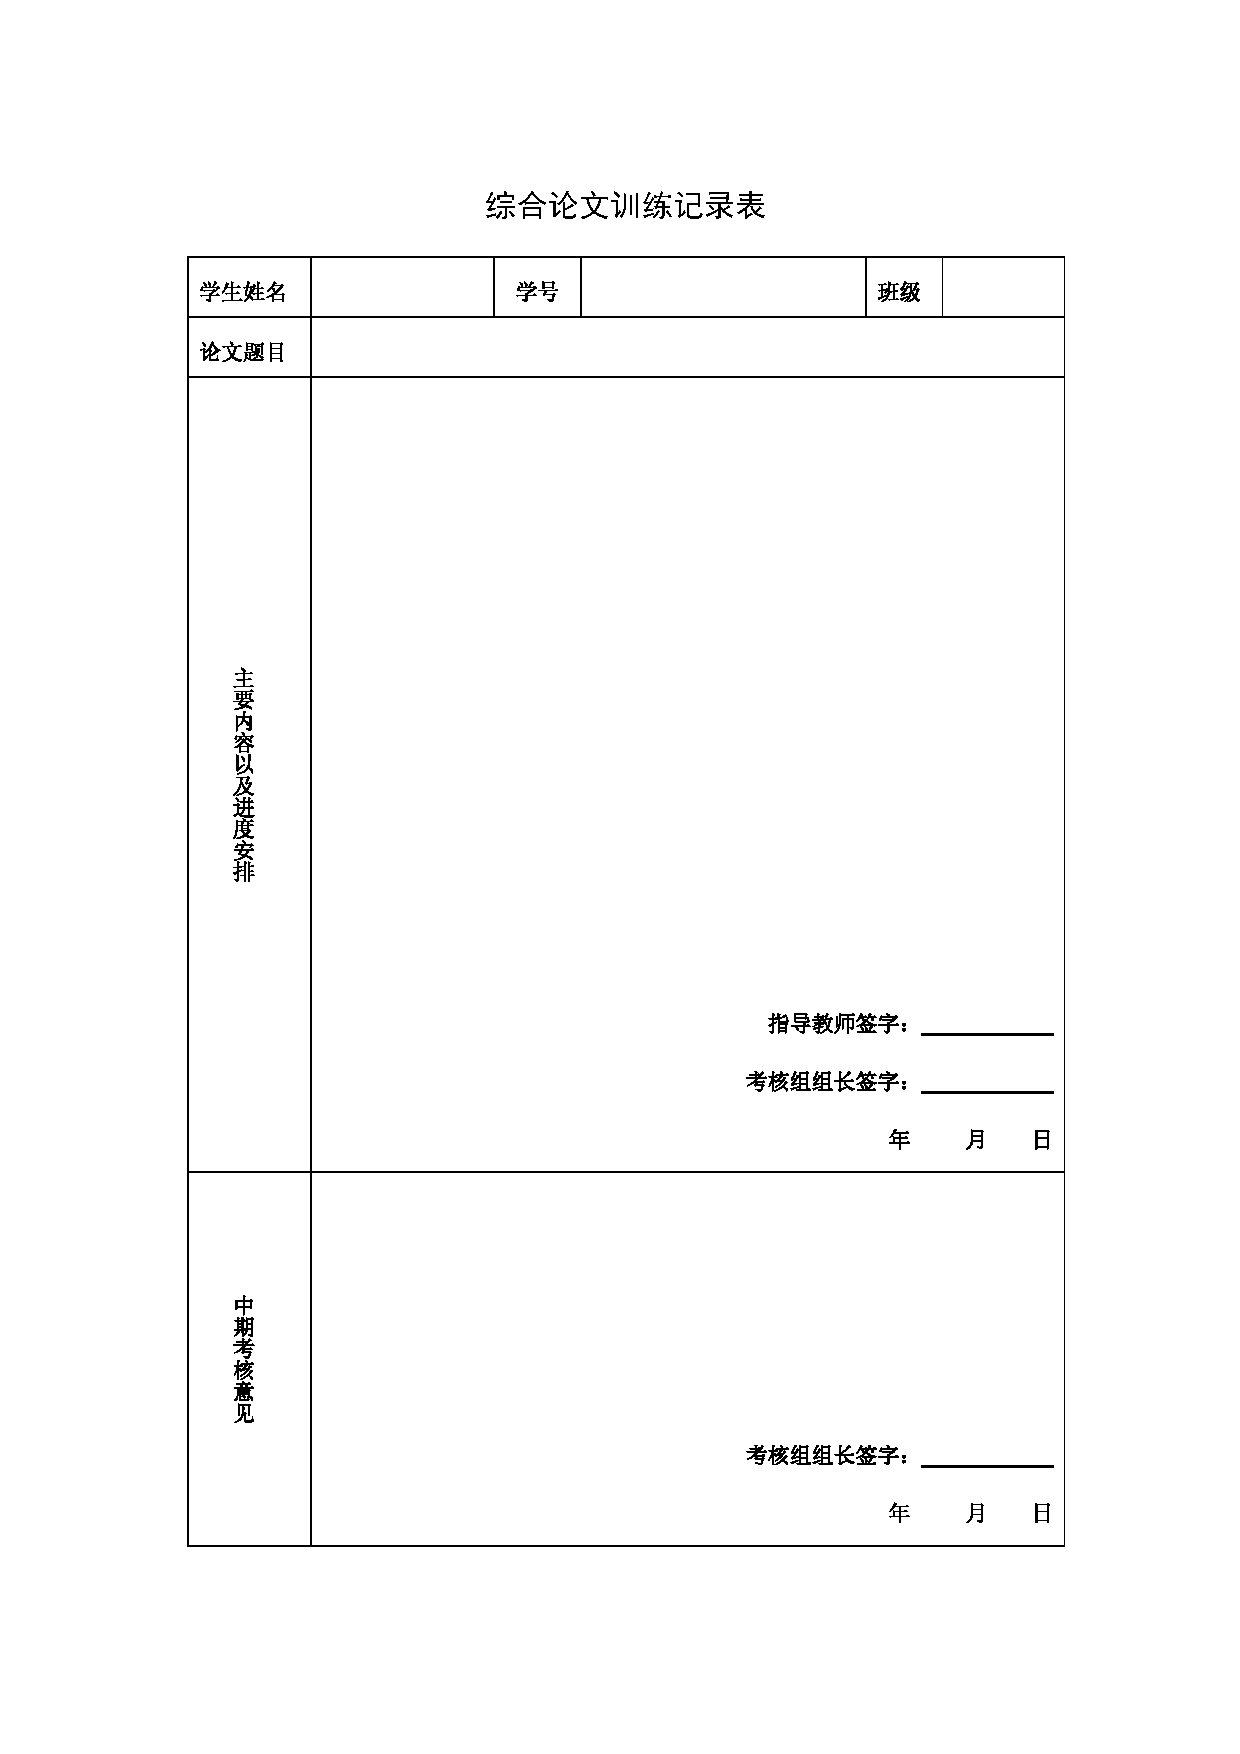
\includepdf[pages=-]{scan-record.pdf}

\end{document}
